\section{Group -- Location -- Climate -- Weather File Access}\label{group-location-climate-weather-file-access}

This group of objects describes the ambient conditions for the simulation.

\subsection{Site:Location}\label{sitelocation}

The location class describes the parameters for the building's location. Only one location is allowed. Weather data file location, if it exists, will override any location data in the IDF. Thus, for an annual simulation, a Location does not need to be entered.

\subsubsection{Inputs}\label{inputs-026}

\paragraph{Field: Name}\label{field-name-025}

This alpha field is used as an identifying field in output reports.

\paragraph{Field: Latitude}\label{field-latitude}

This field represents the latitude (in degrees) of the facility. By convention, North Latitude is represented as positive; South Latitude as negative. Minutes should be represented in decimal fractions of 60. (15' is 15/60 or .25)

\paragraph{Field: Longitude}\label{field-longitude}

This field represents the longitude (in degrees) of the facility. By convention, East Longitude is represented as positive; West Longitude as negative. Minutes should be represented in decimal fractions of 60. (15' is 15/60 or .25)

\paragraph{Field: Time Zone}\label{field-time-zone}

This field represents the time zone of the facility (relative to Greenwich Mean Time or the 0\(^{th}\) meridian). Time zones west of GMT (e.g. North America) are represented as negative; east of GMT as positive. Non-whole hours can be represented in decimal (e.g. 6:30 is 6.5).

\paragraph{Field: Elevation}\label{field-elevation}

This field represents the elevation of the facility in meters (relative to sea level).

Units with their abbreviations are shown in Appendix A. And, as shown in an IDF:

\begin{lstlisting}
Site:Location, DENVER COLORADO, ! Name
   39.75000,                    ! Latitude {N+ S-}
  -104.8700,                    ! Longitude {W- E+}
  -7.000000,                    ! TimeZoneNumber {GMT+/-}
  1610.26;                      ! Elevation {m}
\end{lstlisting}

Most examples in this document include the comment lines that illustrate each data field's value. However, this is not necessary (though it makes the IDF more readable). The previous example could also be:

\begin{lstlisting}
Site:Location, DENVER COLORADO,39.75,-104.87,-7,1610.26;
\end{lstlisting}

\subsection{SizingPeriod:DesignDay}\label{sizingperioddesignday}

The design day input describes the parameters to effect a ``design day'' simulation, often used for load calculations or sizing equipment. Using the values in these fields, EnergyPlus ``creates'' a complete days' worth of weather data (air temperatures, solar radiation, etc.) Normal operation uses the default range multipliers as shown in Figure~\ref{fig:default-daily-range-multiplier-for-design} though users may choose to input their own multiplier schedule. Likewise, normal operation specifies one ``humidity indicating condition'' which is used to calculate the humidity ratio at maximum temperature -- this is used as the constant humidity ratio for the entire day. Again, this can be overridden by specifying a relative humidity schedule or requesting generation of an hourly wet-bulb temperature profile. Multiple design days may be specified.

We refer you to the ASHRAE Handbook of Fundamentals for philosophy of what parameters are important for use as ``design conditions'' in sizing equipment.

\begin{callout}
  In the install, the ``design day files'' are included for the weather file locations that are included (weatherdata folder). All the design day definitions from the ASHRAE design conditions (latest publication date) are included, grouped by WMO region, on the main web site with the weather data. \url{http://www.energyplus.gov/cfm/weather_data.cfm} These files are in ``macro'' form but it is easy to cut and paste the appropriate definition segments. These files include the location information as well as some locations have \textbf{RunPeriodControl:DaylightSavingTime} objects.
\end{callout}

\subsubsection{Inputs}\label{inputs-1-024}

\paragraph{Field: Name}\label{field-name-1-023}

This field, like the location name, is used simply for reporting and identification. This name must be unique among the SizingPeriod names entered.

\paragraph{Field: Month}\label{field-month}

This numeric field specifies the month. That, in conjunction with the day of the month and location information, determines the current solar position and solar radiation values for each hour of the day.

\paragraph{Field: Day of Month}\label{field-day-of-month}

This numeric field specifies the day of the month. That, in conjunction with the month and location information, determines the current solar position and solar radiation values for each hour of the day.

\paragraph{Field: Day Type}\label{field-day-type}

This alpha field specifies the day type for the design day. This value indicates which day profile to use in schedules. For further information, see the Schedule discussion later in this document. (ref: Schedule) Note that two of the possible day types are SummerDesignDay (for cooling) and WinterDesignDay (for heating) -- allowing the user to customize schedules for the design conditions. That is, for design days tagged with a SummerDesignDay type, you can set schedules to be worst or typical schedules for a cooling season.

\paragraph{Field: Maximum Dry-Bulb Temperature}\label{field-maximum-dry-bulb-temperature}

This numeric field should contain the day's maximum dry-bulb temperature in degrees Celsius. (Reference Appendix A of this document for EnergyPlus standard units and abbreviations). The MacroDataSets design day files show extreme temperature for locations as indicated in the ASHRAE HOF design condition tables.

\paragraph{Field: Daily Dry-bulb Temperature Range}\label{field-daily-dry-bulb-temperature-range}

A design day can have a ``high'' temperature and a ``low'' temperature (or can be a constant temperature for each hour of the day). If there is a difference between high and low temperatures, this field should contain the difference from the high to the low. EnergyPlus, by default, distributes this range over the 24 hours in the day as shown in the figure below:

\begin{figure}[hbtp] % fig 6
\centering
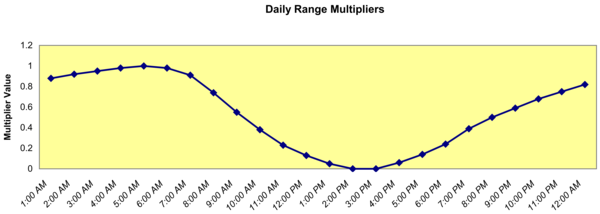
\includegraphics[width=0.9\textwidth, height=0.9\textheight, keepaspectratio=true]{media/image010.png}
\caption{Default Daily range Multiplier for Design Days \protect \label{fig:default-daily-range-multiplier-for-design}}
\end{figure}

The multipliers are taken from the ASHRAE 2009 HOF. More explicitly, EnergyPlus creates an air temperature for each timestep by using the entered maximum dry-bulb temperature in conjunction with the entered daily range and the above multiplier values. The actual equation used is shown below:

\begin{equation}
{T_{current}} = {T_{Max}} - {T_{range}}\cdot {T_{Multiplier}}
\end{equation}

where

T\(_{current}\) = Air temperature of current Hour of Day

T\(_{Max}\) = User supplied Max Dry-bulb Temperature

T\(_{range}\) = User supplied Daily Temperature Range

T\(_{Multiplier}\) = Range multiplier as shown on the above graph

The range multiplier values represent typical conditions of diurnal temperatures (i.e. the low temperature for the day occurring about 5:00 AM and the maximum temperature for the day occurring about 3:00 PM. Note that EnergyPlus does not shift the profile based on the time of solar noon as is optionally allowed in ASHRAE procedures.

ASHRAE research indicates that dry-bulb and wet-bulb temperatures typically follow the same profile, so EnergyPlus can use the default profile to generate humidity conditions (see Humidity Indicating Type = WetBulbProfileDefaultMultipliers below).

\paragraph{Field: Dry-Bulb Temperature Range Modifier Type}\label{field-dry-bulb-temperature-range-modifier-type}

If you are happy with lows at 5am and highs at 3pm, you can ignore this field. If you want to specify your own temperature range multipliers (see earlier discussion at the Temperature Range field description), you can specify a type here and create a day schedule which you reference in the next field.

If you specify \textbf{MultiplierSchedule} in this field, then you need to create a day schedule that specifies a multiplier applied to the temperature range field (above) to create the proper dry-bulb temperature range profile for your design day.

If you specify \textbf{DifferenceSchedule} in this field, then you need to create a day schedule that specifies a number to be \textbf{subtracted} from dry-bulb maximum temperature for each timestep in the day. Note that numbers in the delta schedules cannot be negative as that would result in a higher maximum than the maximum previously specified.

If you specify \textbf{TemperatureProfileSchedule} in this field, then you need to create a day schedule that specifies the actual dry-bulb temperatures throughout the day. You will not need to include a Maximum Dry-Bulb Temperature in that field.

If you leave this field blank or enter \textbf{DefaultMultipliers}, then the default multipliers will be used as shown in the ``temperature range'' field above.

\paragraph{Field: Dry-Bulb Temperature Range Modifier Day Schedule Name}\label{field-dry-bulb-temperature-range-modifier-day-schedule-name}

This field is the name of a \textbf{day schedule} (ref. Schedule:Day:Hourly, Schedule:Day:Interval, Schedule:Day:List objects) with the values as specified in the Dry-Bulb Temperature Range Modifier Type field above.

\paragraph{Field: Humidity Condition Type}\label{field-humidity-condition-type}

The values/schedules indicated here and in subsequent fields create the humidity values in the 24 hour design day conditions profile. Valid choices here are: \textbf{WetBulb}, \textbf{Dewpoint}, \textbf{WetBulbProfileDefaultMultipliers, WetBulbProfileDifferenceSchedule,} \textbf{WetBulbProfileMultiplierSchedule}, \textbf{HumidityRatio}, \textbf{Enthalpy}, and \textbf{Schedule.}

The Humidity Condition Type fields have interacting uses and units, summarized as follows:

% table 2
\begin{longtable}[c]{p{2.25in}p{1.75in}p{2.0in}}
\caption{Humidity Indicating Field Interactions - Design Day \label{table:humidity-indicating-field-interactions-design}} \tabularnewline
\toprule 
Humidity Condition Type & Primary Humidity Indicating Field & Humidity Indicating Day Schedule \tabularnewline
\midrule
\endfirsthead

\caption[]{Humidity Indicating Field Interactions - Design Day} \tabularnewline
\toprule 
Humidity Condition Type & Primary Humidity Indicating Field & Humidity Indicating Day Schedule \tabularnewline
\midrule
\endhead

WetBulb & Wetbulb or DewPoint at Maximum Dry-Bulb & N/A (unused) \tabularnewline
DewPoint & Wetbulb or DewPoint at Maximum Dry-Bulb & N/A (unused) \tabularnewline
HumidityRatio & Humidity Ratio at Maximum Dry-Bulb & N/A (unused) \tabularnewline
Enthalpy & Enthalpy at Maximum Dry-Bulb & N/A (unused) \tabularnewline
WetBulbProfile\-DefaultMultipliers & Wetbulb or DewPoint at Maximum Dry-Bulb & N/A (unused) \tabularnewline
WetBulbProfile\-MultiplierSchedule & Wetbulb or DewPoint at Maximum Dry-Bulb & Fractions of wet-bulb daily range (0 – 1) \tabularnewline
WetBulbProfile\-DifferenceSchedule & Wetbulb or DewPoint at Maximum Dry-Bulb & Difference between maximum and hour/timestep wet-bulb temperature, C \tabularnewline
RelativeHumidity\-Schedule & N/A & Relative humidity (\%, 0 – 100) \tabularnewline
\bottomrule
\end{longtable}

Humidity conditions over the day are derived as follows:

\textbf{WetBulb, DewPoint, HumidityRatio, or Enthalpy}:

These four methods assume constant absolute humidity over the day. Calculate W = humidity ratio at Maximum Dry-Bulb Temperature and Humidity Indicating Conditions. Derive hourly/timestep humidity conditions from W and hour/timestep dry-bulb temperature.

\textbf{WetBulbProfileDefaultMultipliers}

Generate the wet-bulb temperature profile using Default Daily Range Multiplier for Design Days (shown in Figure~\ref{fig:default-daily-range-multiplier-for-design} above) and Daily Wet-Bulb Temperature Range (below). This method is analogous to DefaultMultiplier generation of the dry-bulb temperature profile and is the procedure recommended in Chapter 14 of ASHRAE 2009 HOF.

\textbf{WetBulbProfileMultiplierSchedule}

Generate the wet-bulb profile using multipliers from the Humidity Indicating Day Schedule and Daily Wet-Bulb Temperature Range (below). Analogous to dry-bulb MultiplierSchedule.

\textbf{WetBulbProfileDifferenceSchedule}

Generate the wet-bulb profile by subtracting Humidity Indicating Day Schedule values from the daily maximum wet-bulb temperature (specified in Humidity Indicating Conditions at Maximum Dry-Bulb). Analogous to dry-bulb DifferenceSchedule.

\textbf{RelativeHumiditySchedule}

Hourly relative humidity is specified in Humidity Indicating Day Schedule.

In all cases, the humidity ratio is limited to saturation at the hour/timestep dry-bulb (that is, the dry-bulb temperature is used as specified, but the humidity ratio is modified as needed to be physically possible). Once a valid air state is determined, a complete set of consistent hour/timestep psychrometric values (dewpoint, wet-bulb, and enthalpy) is derived.

\paragraph{Field: Wetbulb or DewPoint at Maximum Dry-Bulb}\label{field-wetbulb-or-dewpoint-at-maximum-dry-bulb}

If you choose \textbf{Wetbulb} or \textbf{Dewpoint} in the Humidity Condition Type field, then this numeric field should contain that value. Note that this field is unnecessary when you put in a humidity indicating day schedule (described later in this section).

\paragraph{Field: Humidity Condition Day Schedule Name}\label{field-humidity-condition-day-schedule-name}

Allows specification a day schedule (ref. Schedule:Day:Hourly, Schedule:Day:Interval, Schedule:Day:List objects) of values for relative humidity or wet-bulb profile per Humidity Indicating Type field.

\paragraph{Field: Humidity Ratio at Maximum Dry-Bulb}\label{field-humidity-ratio-at-maximum-dry-bulb}

If \textbf{HumidityRatio} is chosen for the Humidity Condition Type field, then this numeric field should contain the desired humidity ratio at maximum dry-bulb temperature (units kg Water / kg Dry Air).

\paragraph{Field: Enthalpy at Maximum Dry-Bulb}\label{field-enthalpy-at-maximum-dry-bulb}

If \textbf{Enthalpy} is chosen for the Humidity Condition Type field, then this numeric field should contain the desired enthalpy at maximum dry-bulb temperature (units Joules /kg).

\paragraph{Field: Daily Wet-Bulb Temperature Range}\label{field-daily-wet-bulb-temperature-range}

The difference between the maximum and minimum wet-bulb temperatures on the design day (Celsius). Used for generating daily profiles of humidity conditions when Humidity Condition Type field (above) is \textbf{WetBulbProfileDefaultMultipliers} or \textbf{WetBulbProfileMultiplierSchedule}. Values for wet-bulb temperature range are tabulated by month for 5564 locations worldwide on the CD that accompanies the ASHRAE 2009 HOF.

\paragraph{Field: Barometric Pressure}\label{field-barometric-pressure}

This numeric field is the constant barometric pressure (Pascals) for the entire day.

\paragraph{Field: Wind Speed}\label{field-wind-speed}

This numeric field is the wind speed in meters/second (constant throughout the day) for the day. The MacroDataSets design day files includes wind speed values (99.6\% - heating, 1\% cooling) as indicated in ASHRAE HOF design condition tables. But, you should be aware that traditional values for these are 6.7056 m/s (15 mph) for heating and 3.3528 m/s (7 mph) for cooling. A reminder is shown in the comments for the wind speed values. The comments also note the extreme wind speeds from the ASHRAE tables.

\paragraph{Field: Wind Direction}\label{field-wind-direction}

This numeric field is the source wind direction in degrees. By convention, winds from the North would have a value of 0., from the East a value of 90.

\paragraph{Field: Rain Indicator}\label{field-rain-indicator}

This field indicates whether or not the building surfaces are wet. If the value is Yes, then it is assumed that the building surfaces are wet. Wet surfaces may change the conduction of heat through the surface.

\paragraph{Field: Snow Indicator}\label{field-snow-indicator}

This field indicates whether or not there is snow on the ground. If the value is Yes, then it is assumed there is snow on the ground. Snow on the ground changes the ground reflectance properties.

\paragraph{Field: Daylight Saving Time Indicator}\label{field-daylight-saving-time-indicator}

This field specifies whether to consider this day to be a Daylight Saving Day. Yes in the field indicates that daylight saving time is operational for this day. Yes essentially adds 1 hour to the scheduling times used in items with schedules.

\paragraph{Field: Solar Model Indicator}\label{field-solar-model-indicator}

This field allows the user to select \textbf{ASHRAE\-Clear\-Sky, ASHRAE\-Tau, Zhang\-Huang, or Sche\-dule} for solar modeling in the calculation of the solar radiation in the design day. ASHRAE\-Clear\-Sky and Zhang\-Huang use the Clearness value as part of their calculations. ASHRAE\-Tau invokes the revised model specified in Chapter 14 of the ASHRAE 2009 HOF and uses Taub and Taud values (below). Technical details of the models are described in the Engineering Reference. The \textbf{Schedule} choice allows you to enter schedule values for the day's profile (use the next two fields for the names).

\paragraph{Field: Beam Solar Day Schedule Name}\label{field-beam-solar-day-schedule-name}

This field allows the option for you to put in your own day profile of beam solar values (wh/m2). These values will replace the calculated values during design day processing. Only day schedules (ref. Schedule:Day:Hourly, Schedule:Day:Interval, Schedule:Day:List objects) are used here.

\paragraph{Field: Diffuse Solar Day Schedule Name}\label{field-diffuse-solar-day-schedule-name}

This field allows the option for you to put in your own day profile of diffuse solar values (wh/m2). These values will replace the calculated values during design day processing. Only day schedules (ref. Schedule:Day:Hourly, Schedule:Day:Interval, Schedule:Day:List objects) are used here.

\paragraph{Field: ASHRAE Clear Sky Optical Depth for Beam Irradiance (taub)}\label{field-ashrae-clear-sky-optical-depth-for-beam-irradiance-taub}

Optical depth for beam radiation, used only when Solar Model Indicator is ASHRAETau. See next field.

\paragraph{Field: ASHRAE Clear Sky Optical Depth for Diffuse Irradiance (taud)}\label{field-ashrae-clear-sky-optical-depth-for-diffuse-irradiance-taud}

Optical depth for diffuse radiation, used only when Solar Model Indicator is ASHRAETau. Taub and Taud values are tabulated by month for 5564 locations worldwide on the CD that accompanies the ASHRAE 2009 HOF.

\paragraph{Field: Sky Clearness}\label{field-sky-clearness}

If the choice in the Solar Model Indicator field is ASHRAEClearSky or ZhangHuang, then this numeric field should be entered. This value represents the ``clearness'' value for the day. This value, along with the solar position as defined by the Location information and the date entered for the design day, help define the solar radiation values for each hour of the day. Clearness may range from 0.0 to 1.2, where 1.0 represents a clear sky at sea level. Values greater than 1.0 may be used for high altitude locations. Traditionally, one uses 0.0 clearness for Winter Design Days. Note that this ``sky clearness'' does not have the same meaning as output variable ``Site Daylighting Model Sky Clearness''.

IDF Examples:

\begin{lstlisting}
! Phoenix Sky Harbor Intl Ap_AZ_USA Annual Cooling (WB = >MDB)
!   .4%, MDB = 35.8°C WB = 24.5°C
SizingPeriod:DesignDay,
  Phoenix Sky Harbor Intl Ap Ann Clg .4% Condns WB = >MDB, !- Name
          7,      !- Month
         21,      !- Day of Month
  SummerDesignDay,!- Day Type
       35.8,      !- Maximum Dry-Bulb Temperature {C}
         12,      !- Daily Dry-Bulb Temperature Range {C}
  DefaultMultipliers, !- Dry-Bulb Temperature Range Modifier Type
           ,      !- Dry-Bulb Temperature Range Modifier Schedule Name
    Wetbulb,      !- Humidity Condition Type
       24.5,      !- Wetbulb at Maximum Dry-Bulb {C}
           ,      !- Humidity Indicating Day Schedule Name
           ,      !- Humidity Ratio at Maximum Dry-Bulb {kgWater/kgDryAir}
           ,      !- Enthalpy at Maximum Dry-Bulb {J/kg}
           ,      !- Daily Wet-Bulb Temperature Range {deltaC}
     97342.,      !- Barometric Pressure {Pa}
        4.1,      ! Wind Speed {m/s}
        260,      !- Wind Direction {Degrees; N = 0, S = 180}
         No,      !- Rain {Yes/No}
         No,      !- Snow on ground {Yes/No}
         No,      !- Daylight Savings Time Indicator
       ASHRAETau, !- Solar Model Indicator
           ,      !- Beam Solar Day Schedule Name
           ,      !- Diffuse Solar Day Schedule Name
      0.588,     !- ASHRAE Clear Sky Optical Depth for Beam Irradiance (taub)
      1.653;  !- ASHRAE Clear Sky Optical Depth for Diffuse Irradiance (taud)

SizingPeriod:DesignDay,
  Denver Centennial Golden Ann Htg 99% Condns DB - sched solar,  !- Name
  1,                       !- Month
  13,                      !- Day of Month
  WinterDesignDay,         !- Day Type
  -16,                     !- Maximum Dry-Bulb Temperature {C}
  0.0,                     !- Daily Dry-Bulb Temperature Range {deltaC}
  ,                        !- Dry-Bulb Temperature Range Modifier Type
  ,                    !- Dry-Bulb Temperature Range Modifier Schedule Name
  Wetbulb,                 !- Humidity Condition Type
  -16,                     !- Wetbulb or DewPoint at Maximum Dry-Bulb {C}
  ,                        !- Humidity Indicating Day Schedule Name
  ,               !- Humidity Ratio at Maximum Dry-Bulb {kgWater/kgDryAir}
  ,                        !- Enthalpy at Maximum Dry-Bulb {J/kg}
  ,                        !- Daily Wet-Bulb Temperature Range {deltaC}
  83411.,                  !- Barometric Pressure {Pa}
  2.3,                     !- Wind Speed {m/s}
  180,                     !- Wind Direction {deg}
  No,                      !- Rain Indicator
  No,                      !- Snow Indicator
  No,                      !- Daylight Saving Time Indicator
  Schedule,                !- Solar Model Indicator
  Winter (1/13) Beam Solar,!- Beam Solar Day Schedule Name
  Winter (1/13) Diffuse Solar;  !- Diffuse Solar Day Schedule Name

Schedule:Day:Hourly,
  Winter (1/13) Beam Solar,
  Any Number,
  0,0,0,0,0,0,0,190,698,852,892,919,957,953,856,700,213,0,0,0,0,0,0,0;

Schedule:Day:Hourly,
  Winter (1/13) Diffuse Solar,
  Any Number,
  0,0,0,0,0,0,0,35,118,116,92,65,40,14,0,0,5,0,0,0,0,0,0,0;
\end{lstlisting}

Look at the example files 1Zone\-Un\-controll\-ed\_\-DD\-Changes.idf and 1Zone\-Un\-controlled\_\-DD\-2009 for several examples of specifying Design Day inputs.

\subsubsection{Outputs}\label{outputs-018}

For the schedule fields in the object, several output variables can be used:

\begin{itemize}
\item
  Zone,Average,Sizing Period Site Beam Solar Schedule Value {[}W/m2{]}
\item
  Zone,Average,Sizing Period Site Diffuse Solar Schedule Value {[}W/m2{]}
\item
  Zone,Average,Sizing Period Site Humidity Condition Schedule Value {[}\%{]}
\item
  Zone,Average,Sizing Period Site Humidity Condition Schedule Value {[]}
\item
  Zone,Average,Sizing Period Site Drybulb Temperature Range Modifier Schedule Value {[]}
\item
  Zone,Average,Sizing Period Site Drybulb Temperature Range Modifier Schedule Value {[}deltaC{]}
\item
  Zone,Average,Sizing Period Site Drybulb Temperature Range Modifier Schedule Value {[}C{]}
\item
  Zone,Average,Sizing Period Site Sky Temperature Schedule Value {[}deltaC{]}
\item
  Zone,Average,Sizing Period Site Sky Temperature Schedule Value {[}C{]}
\end{itemize}

\paragraph{Sizing Period Site Beam Solar Schedule Value {[}W/m2{]}}\label{sizing-period-site-beam-solar-schedule-value-wm2}

\paragraph{Sizing Period Site Diffuse Solar Schedule Value {[}W/m2{]}}\label{sizing-period-site-diffuse-solar-schedule-value-wm2}

This schedule value is active when any Design Day objects have / use the solar schedule option. For those objects that don't have this option, the value will be displayed as -999.

\paragraph{Sizing Period Site Humidity Condition Schedule Value {[}\%{]}}\label{sizing-period-site-humidity-condition-schedule-value}

\paragraph{Sizing Period Site Humidity Condition Schedule Value {[]}}\label{sizing-period-site-humidity-condition-schedule-value-1}

This schedule value is active when any Design Day objects have / use the humidity schedule option. For those objects that don't have this option, the value will be displayed as -999.

\paragraph{Sizing Period Site Drybulb Temperature Range Modifier Schedule Value {[]}}\label{sizing-period-site-drybulb-temperature-range-modifier-schedule-value}

\paragraph{Sizing Period Site Drybulb Temperature Range Modifier Schedule Value {[}deltaC{]}}\label{sizing-period-site-drybulb-temperature-range-modifier-schedule-value-deltac}

\paragraph{Sizing Period Site Drybulb Temperature Range Modifier Schedule Value {[}C{]}}\label{sizing-period-site-drybulb-temperature-range-modifier-schedule-value-c}

This schedule value is active when any Design Day objects have / use the drybulb temperature range modifier schedule option. For those objects that don't have this option, the value will be displayed as -999.

\paragraph{Sizing Period Site Sky Temperature Schedule Value {[}deltaC{]}}\label{sizing-period-site-sky-temperature-schedule-value-deltac}

\paragraph{Sizing Period Site Sky Temperature Schedule Value {[}C{]}}\label{sizing-period-site-sky-temperature-schedule-value-c}

This schedule value is active when any Design Day objects have / use the WeatherProperties:SkyTemperature schedule option. For those objects that don't have this option, the value will be displayed as -999.

\subsection{Longer Design Periods}\label{longer-design-periods}

Some features may benefit by using a longer design weather period for sizing or loads calculations. Longer design periods may be created by using the \textbf{Si\-zing\-Period:\-Weather\-File\-Days} or \textbf{Si\-zing\-Period:\-Weather\-File\-Con\-dition\-Type} objects. These two objects allow for selections from an attached weather file to be used in the sizing calculations.

\subsection{Sizing\-Period:\-Weather\-File\-Days}\label{sizingperiodweatherfiledays}

The Sizing\-Period:\-Weather\-File\-Days object describes using a selected period from the ``attached'' weather file to be used in load calculations or sizing equipment. The period selected can be as small as a single day or larger. Multiple periods may be input. While this object may be used for sizing calculations, you should also consider using design days that represent more long term extremes or conditions.

\subsubsection{Inputs}\label{inputs-2-022}

\paragraph{Field: Name}\label{field-name-2-021}

This field allows for an assigned name for this run period so it can be tracked easily in sizing and other outputs.

\paragraph{Field: Begin Month}\label{field-begin-month}

This numeric field should contain the starting month number (1 = January, 2 = February, etc.) for the annual run period desired.

\paragraph{Field: Begin Day of Month}\label{field-begin-day-of-month}

This numeric field should contain the starting day of the starting month (must be valid for month) for the annual run period desired.

\paragraph{Field: End Month}\label{field-end-month}

This numeric field should contain the ending month number (1 = January, 2 = February, etc.) for the annual run period desired.

\paragraph{Field: End Day of Month}\label{field-end-day-of-month}

This numeric field should contain the ending day of the ending month (must be valid for month) for the annual run period desired.

\paragraph{Field: Day of Week for Start Day}\label{field-day-of-week-for-start-day}

For flexibility, the day of week indicated on the weather file can be overridden by this field's value. Valid days of the week (Sunday, Monday, Tuesday, Wednesday, Thursday, Friday, Saturday) or special days (SummerDesignDay, WinterDesignDay, CustomDay1, CustomDay2) must be entered in this field. To clarify, this value will be used as the Start Day (type) for this sizing period. When weekdays are used, each subsequent day in the period will be incremented. When SummerDesignDay, WinterDesignDay, CustomDay1, CustomDay2 -- are used, the day type will be applied for the entire period.

\paragraph{Field: Use Weather File Daylight Saving Period}\label{field-use-weather-file-daylight-saving-period}

Weather files can contain indicators of Daylight Saving Period days. For flexibility, you may want to ignore these designations on the weather file. This field should contain the word \textbf{Yes} if you will accept daylight saving period days as contained on the weather file (note: not all weather files may actually have this period) or \textbf{No} if you wish to ignore Daylight Saving Period days that may be on the weather file.

Note that a blank or null field in this field will indicate \textbf{Yes}.

\paragraph{Field: Use Weather File Rain and Snow Indicators}\label{field-use-weather-file-rain-and-snow-indicators}

Weather files can contain ``rain'' and ``snow'' indicators. (EPW field ``Present Weather Codes'' -- described in the AuxiliaryPrograms document). In turn, rain indicates wet surfaces which changes the film convection coefficient for the surface. Other models may use rain as well (Ground Heat Exchangers). Snow indicators can change the ground reflectance if there is snow on the ground. Entering ``\textbf{Yes}'' in this field allows the weather file conditions to represent ``Rain'' and ``Snow''; entering ``\textbf{No}'' in the field ``turns off'' the rain/snow indicators for this period. You might use this to be able to compare two ``same location'' weather files of different years, origins, etc.

IDF Example:

\begin{lstlisting}
SizingPeriod:WeatherFileDays,
  Summer including Extreme Summer days, !- Name
  7,18,7,25,                            !- Begin/end Day/Month
  SummerDesignDay,                      !- Day type
  No,                                   !- Use Weather File Daylight Saving Period
  No;                                   !- Use Weather File Rain and Snow Indicators

SizingPeriod:WeatherFileDays,
  Winter including Extreme Winter days, !- Name
  1,25,2,1,                             !- Begin/end Day/Month
  WinterDesignDay,                      !- Day type
  No,                                   !- Use Weather File Daylight Saving Period
  No;                                   !- Use Weather File Rain and Snow Indicators
\end{lstlisting}

\subsection{Sizing\-Period:\-Weather\-File\-Con\-dition\-Type}\label{sizingperiodweatherfileconditiontype}

When the EPW files are created, a heuristic procedure identifies extreme and typical periods in the actual weather file. This object will allow one of those periods to be selected for sizing or load calculations (typically). Multiple objects may be input. While this object may be used for sizing calculations, you should also consider using design days that represent more long term extremes or conditions.

\subsubsection{Inputs}\label{inputs-3-020}

\paragraph{Field: Name}\label{field-name-3-018}

This field allows for an assigned name for this run period so it can be tracked easily in sizing and other outputs.

\paragraph{Field: Period Selection}\label{field-period-selection}

This field allows the generic period calculated from the weather file to be selected for this run period. It is not completely generic as there may be extreme cold periods in some weather files but extreme wet periods (tropical) in others. Not all weather files have all of the valid choices. The choices for this field are:

\begin{itemize}
\item
  SummerExtreme
\item
  SummerTypical
\item
  WinterExtreme
\item
  WinterTypical
\item
  AutumnTypical
\item
  SpringTypical
\item
  WetSeason
\item
  DrySeason
\item
  NoDrySeason
\item
  NoWetSeason
\item
  TropicalHot
\item
  TropicalCold
\end{itemize}

\paragraph{Field: Day of Week for Start Day}\label{field-day-of-week-for-start-day-1}

For flexibility, the day of week indicated on the weather file can be overridden by this field's value. Valid days of the week (Sunday, Monday, Tuesday, Wednesday, Thursday, Friday, Saturday) or special days (SummerDesignDay, WinterDesignDay, CustomDay1, CustomDay2) must be entered in this field. To clarify, this value will be used as the Start Day (type) for this sizing period. When weekdays are used, each subsequent day in the period will be incremented. When SummerDesignDay, WinterDesignDay, CustomDay1, CustomDay2 -- are used, the day type will be applied for the entire period.

\paragraph{Field: Use Weather File Daylight Saving Period}\label{field-use-weather-file-daylight-saving-period-1}

Weather files can contain indicators of Daylight Saving Period days. For flexibility, you may want to ignore these designations on the weather file. This field should contain the word \textbf{Yes} if you will accept daylight saving period days as contained on the weather file (note: not all weather files may actually have this period) or \textbf{No} if you wish to ignore Daylight Saving Period days that may be on the weather file.

Note that a blank or null field in this field will indicate \textbf{Yes}.

\paragraph{Field: Use Weather File Rain and Snow Indicators}\label{field-use-weather-file-rain-and-snow-indicators-1}

Weather files can contain ``rain'' and ``snow'' indicators. (EPW field ``Present Weather Codes'' -- described in the AuxiliaryPrograms document). In turn, rain indicates wet surfaces which changes the film convection coefficient for the surface. Other models may use rain as well (Ground Heat Exchangers). Snow indicators can change the ground reflectance if there is snow on the ground. Entering ``\textbf{Yes}'' in this field allows the weather file conditions to represent ``Rain'' and ``Snow''; entering ``\textbf{No}'' in the field ``turns off'' the rain/snow indicators for this period. You might use this to be able to compare two ``same location'' weather files of different years, origins, etc.

IDF Example:

\begin{lstlisting}
SizingPeriod:WeatherFileConditionType,
  Extreme Summer Weather Period for Design, !- Name
  SummerExtreme,                            !- Period Selection
  SummerDesignDay,                          !- Day Type
  No,                                       !- Use Weather File Daylight Saving Period
  No;                                       !- Use Weather File Rain and Snow Indicators

SizingPeriod:WeatherFileConditionType,
  Extreme Winter Weather Period for Design, !- Name
  WinterExtreme,                            !- Period Selection
  WinterDesignDay,                          !- Day Type
  No,                                       !- Use Weather File Daylight Saving Period
  No;                                       !- Use Weather File Rain and Snow Indicators
\end{lstlisting}

\subsection{RunPeriod}\label{runperiod}

The RunPeriod object describes the elements necessary to create a weather file simulation. Multiple run periods may be input. EnergyPlus accepts weather files in the special EnergyPlus weather format (described briefly below this document and in more detail in the Auxiliary Programs document). These files can describe Daylight Saving Time periods as well as holidays within their definitions. The RunPeriod object allows the user to override the use of both the Daylight Saving Period (i.e. use or ignore) and holidays that are embedded within the weather file. Note that the weather file also may contain design condition information, typical and extreme period information, ground temperatures based on air temperature calculations.

\subsubsection{Inputs}\label{inputs-4-018}

\paragraph{Field: Name}\label{field-name-4-015}

This optional field allows the RunPeriod to be named for output reporting. When left blank, the weather file location name is used. Note that the weather file location name will be appended to this name in tabular/summary reports.

\paragraph{Field: Begin Month}\label{field-begin-month-1}

This numeric field should contain the starting month number (1 = January, 2 = February, etc.) for the annual run period desired.

\paragraph{Field: Begin Day of Month}\label{field-begin-day-of-month-1}

This numeric field should contain the starting day of the starting month (must be valid for month) for the annual run period desired.

\paragraph{Field: End Month}\label{field-end-month-1}

This numeric field should contain the ending month number (1 = January, 2 = February, etc.) for the annual run period desired.

\paragraph{Field: End Day of Month}\label{field-end-day-of-month-1}

This numeric field should contain the ending day of the ending month (must be valid for month) for the annual run period desired.

\paragraph{Field: Day of Week for Start Day}\label{field-day-of-week-for-start-day-2}

For flexibility, the day of week indicated on the weather file can be overridden by this field's value. Valid days of the week (Sunday, Monday, Tuesday, Wednesday, Thursday, Friday, Saturday) must be entered in this field. To clarify, this value will be used as the Start Day (type) for this run period and subsequent days will be implemented. If a blank or UseWeatherFile is entered here, then the starting day type will be calculated from the weather file (ref: Auxiliary Programs document about Data Periods).

\paragraph{Field: Use Weather File Holidays and Special Days}\label{field-use-weather-file-holidays-and-special-days}

Weather files can contain holiday designations or other kinds of special days. These day types cause a corresponding day's schedule (see SCHEDULE definitions below) to be used during that day. This field should contain the word \textbf{Yes} if holidays or other special days indicated directly on the weather file should retain their ``day type'' or \textbf{No} if holidays or other special days on the weather file should be ignored. Reference the RunPeriodControl:SpecialDays object below to enter your own special days and holidays.

Note that a blank or null field in this field will indicate \textbf{Yes}.

\paragraph{Field: Use Weather File Daylight Saving Period}\label{field-use-weather-file-daylight-saving-period-2}

Weather files can contain indicators of Daylight Saving period days. For flexibility, you may want to ignore these designations on the weather file. This field should contain the word \textbf{Yes} if you will accept daylight saving period days as contained on the weather file (note: not all weather files may actually have this period) or \textbf{No} if you wish to ignore Daylight Saving period days that may be on the weather file.

Note that a blank or null field in this field will indicate \textbf{Yes}.

\paragraph{Field: Apply Weekend Holiday Rule}\label{field-apply-weekend-holiday-rule}

In some countries (notably the US), when holidays fall on weekends, they are often observed on a weekday close to the holiday day. (Usually if the specific day falls on a Saturday, the observed day is Friday; if on a Sunday, the observed day is Monday). EnergyPlus will represent this custom using the value in this field. If the field is \textbf{Yes}, then specific date holidays that have a duration of one day, will be ``observed'' on the Monday after the day. (Specific day holidays are such as January 1 -- a day-month combination). If the field is blank or \textbf{No}, then the holiday will be shown on the day-month as entered. As this option is listed at the RunPeriod, all applicable special days for the run will use the rule -- there is no override for individual special days.

Note that a blank or null field in this field will indicate \textbf{No}.

\begin{callout}
Note: EnergyPlus processed weather files available on the EnergyPlus web site: \url{http://www.energyplus.gov/cfm/weather\_data.cfm} have neither special days specified nor daylight saving period. However, DDY (Design Day) files produced from the ASHRAE Design Conditions that accompany the EPW files may include a DaylightSavingPeriod object for certain locations.
\end{callout}

\paragraph{Field: Use Weather File Rain Indicators}\label{field-use-weather-file-rain-indicators}

Weather files can contain ``rain'' indicators. (EPW field ``Present Weather Codes'' -- described in the AuxiliaryPrograms document). In turn, rain indicates wet surfaces which changes the film convection coefficient for the surface. Other models may use rain as well (Ground Heat Exchangers). Entering ``\textbf{Yes}'' in this field allows the weather file conditions to represent ``Rain''; entering ``\textbf{No}'' in the field ``turns off'' the rain indicator for this period. You might use this to be able to compare two ``same location'' weather files of different years, origins, etc.

\paragraph{Field: Use Weather File Snow Indicators}\label{field-use-weather-file-snow-indicators}

Weather files can contain ``snow'' indicators. (EPW field ``Snow Depth'' \textgreater{} 0 indicates ``Snow on the ground''). In turn, snow changes the reflectivity of the ground and cascades changes of this reflectivity. Entering ``\textbf{Yes}'' in this field allows the weather file conditions to represent ``Snow''; entering ``\textbf{No}'' in the field ``turns off'' the snow indicator for this period. You might use this to be able to compare two ``same location'' weather files of different years, origins, etc.

\paragraph{Field: Number of Times Runperiod to be Repeated}\label{field-number-of-times-runperiod-to-be-repeated}

This numeric field represents the number of times (usually years) the simulation has to be carried out in a multi runperiod simulation. The default value is set to 1. The number of years of simulation, in case of a Ground Loop Heat Exchanger (GLHE) simulation, should be equal to the length of simulation field in GLHE object. Note that you can specify a number of simulation years with a shorter run period (e.g. 1 week) and EnergyPlus will repeat the simulation of the shorter run period for that many times. Note that repeating will work with any weather file that contains the start date and end date in a ``Data Period'' (refer to Auxiliary Programs document for more documentation on weather file contents).

\paragraph{Field: Increment Day of Week on Repeat}\label{field-increment-day-of-week-on-repeat}

When repeating RunPeriods (see previous field), you can choose to increment the day of week at the end of the period to have a more continuous day type. Enter \textbf{Yes} to increment the day of the week (default). An entry of \textbf{No} will keep the same day of week values as in the first time through.

\paragraph{Field: Start Year}\label{field-start-year}

When repeating a period, you might (for whatever reason), choose to have a specific year as a starting year. Enter an appropriate 4 digit year in this field. Refer to Auxiliary Programs document for more documentation on weather file contents, particularly in using leap year data (or not) within weather files.

And, as shown in an IDF:

\begin{lstlisting}
RunPeriod,  ! Winter Simulation
  Winter Simulation,  !- Name
  12,  !- Begin Month
  1,  !- Begin Day of Month
  3,  !- End Month
  31,  !- End Day of Month
  UseWeatherFile,  !- Day of Week for Start Day
  Yes,  !- Use Weather File Holidays and Special Days
  Yes,  !- Use Weather File Daylight Saving Period
  No,  !- Apply Weekend Holiday Rule
  Yes,  !- Use Weather File Rain Indicators
  Yes;  !- Use Weather File Snow Indicators

! Multiple year simulation example
RunPeriod,
  Multiple Years,  !- Name
  1,    !- Begin Month
  1,    !- Begin Day of Month
  12,   !- End Month
  31,   !- End Day of Month
  UseWeatherFile,  !- Day of Week for Start Day
  Yes,  !- Use Weather File Holidays and Special Days
  Yes,  !- Use Weather File Daylight Saving Period
  No,   !- Apply Weekend Holiday Rule
  Yes,  !- Use Weather File Rain Indicators
  Yes,  !- Use Weather File Snow Indicators
  3;    !- Number of Times Runperiod to be Repeated
\end{lstlisting}

\subsection{RunPeriod:CustomRange}\label{runperiodcustomrange}

The RunPeriod:CustomRange object describes the elements necessary to use a specially crafted (likely multiple year) weather file in a simulation. These kinds of weather files and simulations might be useful for matching utility periods or simulating several years of differing weather data. Multiple run periods may be input. EnergyPlus accepts weather files in the special EnergyPlus weather format (described briefly below this document and in more detail in the Auxiliary Programs document). In order to effectively use this object, however, you will need to use a text editor (EnergyPlus weather files area simple text files) or possibly a spreadsheet program and then save to a csv (comma separated variable) file. Weather files can describe Daylight Saving Time periods as well as holidays within their definitions. The RunPeriod:CustomRange object allows the user to override the use of both the Daylight Saving Period (i.e. use or ignore) and holidays that are embedded within the weather file. Note that the weather file also may contain design condition information, typical and extreme period information, ground temperatures based on air temperature calculations.

\subsubsection{Inputs}\label{inputs-5-016}

\paragraph{Field: Name}\label{field-name-5-012}

This optional field allows the RunPeriod to be named for output reporting. When left blank, the weather file location name is used. Note that the weather file location name will be appended to this name in tabular/summary reports.

\paragraph{Field: Begin Month}\label{field-begin-month-2}

This numeric field should contain the starting month number (1 = January, 2 = February, etc.) for the annual run period desired.

\paragraph{Field: Begin Day of Month}\label{field-begin-day-of-month-2}

This numeric field should contain the starting day of the starting month (must be valid for month) for the annual run period desired.

\paragraph{Field: Begin Year}\label{field-begin-year}

This numeric field should contain the beginning year for the custom range. Though all EnergyPlus (EPW) weather files contain a year/year field, the RunPeriod object does not use this field (previous object). The \textbf{RunPeriod:CustomRange} object causes the program to look specifically for the begin date specified by these three fields (i.e. Begin Month, Begin Day of Month, Begin Year).

\paragraph{Field: End Month}\label{field-end-month-2}

This numeric field should contain the ending month number (1 = January, 2 = February, etc.) for the annual run period desired.

\paragraph{Field: End Day of Month}\label{field-end-day-of-month-2}

This numeric field should contain the ending day of the ending month (must be valid for month) for the annual run period desired.

\paragraph{Field: End Year}\label{field-end-year}

This numeric field should contain the end year for the custom range. Though all EnergyPlus (EPW) weather files contain a year/year field, the RunPeriod object does not use this field (previous object). The \textbf{RunPeriod:CustomRange} object causes the program to look specifically for the end date specified by these three fields (i.e. End Month, End Day of Month, End Year).

\paragraph{Field: Day of Week for Start Day}\label{field-day-of-week-for-start-day-3}

For flexibility, the day of week indicated on the weather file can be overridden by this field's value. Valid days of the week (Sunday, Monday, Tuesday, Wednesday, Thursday, Friday, Saturday) must be entered in this field. To clarify, this value will be used as the Start Day (type) for this run period and subsequent days will be implemented. If a blank or UseWeatherFile is entered here, then the starting day type will be calculated from the weather file (ref: Auxiliary Programs document about Data Periods).

\paragraph{Field: Use Weather File Holidays and Special Days}\label{field-use-weather-file-holidays-and-special-days-1}

Weather files can contain holiday designations or other kinds of special days. These day types cause a corresponding day's schedule (see SCHEDULE definitions below) to be used during that day. This field should contain the word \textbf{Yes} if holidays or other special days indicated directly on the weather file should retain their ``day type'' or \textbf{No} if holidays or other special days on the weather file should be ignored. Reference the RunPeriodControl:SpecialDays object below to enter your own special days and holidays.

Note that a blank or null field in this field will indicate \textbf{Yes}.

\paragraph{Field: Use Weather File Daylight Saving Period}\label{field-use-weather-file-daylight-saving-period-3}

Weather files can contain indicators of Daylight Saving period days. For flexibility, you may want to ignore these designations on the weather file. This field should contain the word \textbf{Yes} if you will accept daylight saving period days as contained on the weather file (note: not all weather files may actually have this period) or \textbf{No} if you wish to ignore Daylight Saving period days that may be on the weather file.

Note that a blank or null field in this field will indicate \textbf{Yes}.

\paragraph{Field: Apply Weekend Holiday Rule}\label{field-apply-weekend-holiday-rule-1}

In some countries (notably the US), when holidays fall on weekends, they are often observed on a weekday close to the holiday day. (Usually if the specific day falls on a Saturday, the observed day is Friday; if on a Sunday, the observed day is Monday). EnergyPlus will represent this custom using the value in this field. If the field is \textbf{Yes}, then specific date holidays that have a duration of one day, will be ``observed'' on the Monday after the day. (Specific day holidays are such as January 1 -- a day-month combination). If the field is blank or \textbf{No}, then the holiday will be shown on the day-month as entered. As this option is listed at the RunPeriod, all applicable special days for the run will use the rule -- there is no override for individual special days.

Note that a blank or null field in this field will indicate \textbf{No}.

\begin{callout}
Note: EnergyPlus processed weather files available on the EnergyPlus web site: \url{http://www.energyplus.gov/cfm/weather\_data.cfm} have neither special days specified nor daylight saving period. However, DDY (Design Day) files produced from the ASHRAE Design Conditions that accompany the EPW files may include a DaylightSavingPeriod object for certain locations.
\end{callout}

\paragraph{Field: Use Weather File Rain Indicators}\label{field-use-weather-file-rain-indicators-1}

Weather files can contain ``rain'' indicators. (EPW field ``Present Weather Codes'' -- described in the AuxiliaryPrograms document). In turn, rain indicates wet surfaces which changes the film convection coefficient for the surface. Other models may use rain as well (Ground Heat Exchangers). Entering ``\textbf{Yes}'' in this field allows the weather file conditions to represent ``Rain''; entering ``\textbf{No}'' in the field ``turns off'' the rain indicator for this period. You might use this to be able to compare two ``same location'' weather files of different years, origins, etc.

\paragraph{Field: Use Weather File Snow Indicators}\label{field-use-weather-file-snow-indicators-1}

Weather files can contain ``snow'' indicators. (EPW field ``Snow Depth'' \textgreater{} 0 indicates ``Snow on the ground''). In turn, snow changes the reflectivity of the ground and cascades changes of this reflectivity. Entering ``\textbf{Yes}'' in this field allows the weather file conditions to represent ``Snow''; entering ``\textbf{No}'' in the field ``turns off'' the snow indicator for this period. You might use this to be able to compare two ``same location'' weather files of different years, origins, etc.

\subsection{RunPeriodControl:SpecialDays}\label{runperiodcontrolspecialdays}

For weather file run periods, special day run periods can be described. These will always be in effect for the selected days in the run period. Depending on the Use Special Days value in the RunPeriod:* object(s), these can augment any special days included on the weather file.

\begin{callout}
Note: EnergyPlus processed weather files available on the EnergyPlus web site: \url{http://www.energyplus.gov/cfm/weather\_data.cfm} have neither special days specified nor daylight saving period. However, DDY (Design Day) files produced from the ASHRAE Design Conditions that accompany the EPW files may include a DaylightSavingPeriod object for certain locations.
\end{callout}

\subsubsection{Inputs}\label{inputs-6-013}

\paragraph{Field: Name}\label{field-name-6-010}

This alpha field is the title for the special day period. It must be unique among all the special day period objects entered.

\paragraph{Field: Start Date}\label{field-start-date}

This field is the starting date for the special day period. Dates in this field can be entered in several ways as shown in the accompanying table:

% table 3
\begin{longtable}[c]{@{}ll@{}}
\caption{Date Field Interpretation \label{table:date-field-interpretation}} \tabularnewline
\toprule 
Field Contents & Interpretation \tabularnewline
\midrule
\endfirsthead

\caption[]{Date Field Interpretation} \tabularnewline
\toprule 
Field Contents & Interpretation \tabularnewline
\midrule
\endhead

< number >  /  < number > & Month / Day \tabularnewline
< number >  Month & Day and Month \tabularnewline
Month  < number > & Day and Month \tabularnewline
< number >  Weekday in Month & Numbered weekday of month \tabularnewline
Last Weekday In Month & Last weekday of month \tabularnewline
\bottomrule
\end{longtable}

In the table, Month can be one of (January, February, March, April, May, June, July, August, September, October, November, December). Abbreviations of the first three characters are also valid.

In the table, Weekday can be one of (Sunday, Monday, Tuesday, Wednesday, Thursday, Friday, Saturday). Abbreviations of the first three characters are also valid.

\paragraph{Field: Duration}\label{field-duration}

This numeric field specifies how long (number of days) the special day period lasts.

\paragraph{Field: Special Day Type}\label{field-special-day-type}

This alpha field designates the ``day type'' for schedule use during the special period. It must be one of (Holiday, SummerDesignDay, WinterDesignDay, CustomDay1, CustomDay2).

An example in the IDF would be:

\begin{lstlisting}
RunPeriodControl:SpecialDays, President’s Day, 3rd Monday in February,1,Holiday;
RunPeriodControl:SpecialDays, Thanksgiving, 4th Thursday in November, 1,Holiday;
RunPeriodControl:SpecialDays, Halloween, 10/31, 1, Holiday;
RunPeriodControl:SpecialDays, Vacation, 5/1, 14, CustomDay1;
\end{lstlisting}

\subsection{RunPeriodControl:DaylightSavingTime}\label{runperiodcontroldaylightsavingtime}

Similar to a special day period, a daylight saving period may be entered to be applied to weather file run periods. These will always be in effect, regardless of the value entered on the RunPeriod object. Note that this period will always override any daylight saving period specified in a weather file.

\begin{callout}
Note: EnergyPlus processed weather files available on the EnergyPlus web site: \url{http://www.energyplus.gov/cfm/weather\_data.cfm} have neither special days specified nor daylight saving period.

\warning{Note: For EnergyPlus Output:Variable and Output:Meter reporting, the time stamps are always in standard time. When daylight saving time is active, scheduled loads and controls will shift one hour relative to standard time.}
\end{callout}

\subsubsection{Inputs}\label{inputs-7-013}

\paragraph{Field: Start Date}\label{field-start-date-1}

This is the starting date of the daylight saving period. Note that it can be entered in several formats as shown in Table~\ref{table:date-field-interpretation}. Date Field Interpretation.

\paragraph{Field: End Date}\label{field-end-date}

This is the ending date of the daylight saving period. Note that it can be entered in several formats as shown in Table~\ref{table:date-field-interpretation}. Date Field Interpretation.

And in the IDF:

\begin{lstlisting}
! U.S. Standard for Daylight Saving
RunPeriodControl:DaylightSavingTime,2nd Sunday in March, 1st Sunday in November; !2007
! Brazil standard
RunPeriodControl:DaylightSavingTime,1st Sunday in October, Last Sunday in February;
! European Standard
RunPeriodControl:DaylightSavingTime, Last Sunday in March, Last Sunday in October;
! Syria Standard
RunPeriodControl:DaylightSavingTime, 4/1, 10/1;
\end{lstlisting}

Of course, these could not all appear in the same IDF as only one DaylightSavingPeriod object per input file is allowed. More information on Daylight Saving Periods can be seen on the web at: \url{http://www.webexhibits.org/daylightsaving/}. The ASHRAE Handbook of Fundamentals {[}ASHRAE 2005{]} also contains information about daylight saving periods and their climatic information now includes start and end dates for many locations.

\subsection{WeatherProperty:SkyTemperature}\label{weatherpropertyskytemperature}

Sky Temperature, or radiative sky temperature, is internally calculated by EnergyPlus using an algorithm using horizontal infrared radiation from sky, cloudiness factors and current temperature. The algorithm is fully described in the Engineering Reference document. For flexibility, the following object can be entered to override the internal calculations. Much of the literature describes the sky temperature as relative to either drybulb or dewpoint temperature.

\subsubsection{Inputs}\label{inputs-8-011}

\paragraph{Field: Name}\label{field-name-7-009}

This name references an existing design period (i.e., SizingPeriod:DesignDay, SizingPeriod:WeatherFileDays, or SizingPeriod:WeatherFileConditionType) or run period (by name or blank for all run periods).

\paragraph{Field: Calculation Type}\label{field-calculation-type}

Allowable entries here are: \textbf{ScheduleValue}, \textbf{DifferenceScheduleDryBulbValue}, or \textbf{DifferenceScheduleDewPointValue}. In each case the following field must specify a valid schedule name. \textbf{ScheduleValue} -- the values in the schedule are used as the sky temperature. \textbf{DifferenceScheduleDryBulbValue} -- the values in the schedule are used as a difference to the drybulb temperature value (+values would then be greater than the drybulb temperature, -values would then be less than the drybulb temperature) for the resulting sky temperature value. \textbf{DifferenceScheduleDewPointValue} -- the values in the schedule are used as a difference to the dewpoint temperature value (+values would then be greater than the dewpoint temperature, -values would then be less than the dewpoint temperature) for the resulting sky temperature value.

\paragraph{Field: ScheduleName}\label{field-schedulename}

This field specifies a schedule name to accomplish the sky temperature calculation from the previous field. A Schedule:Day:* (i.e., Schedule:Day:Hourly, Schedule:Day:Interval, Schedule:Day:List) should be specified if the name in the name field matches a SizingPeriod:DesignDay object. If the name is one of the weather file period specifications (i.e. matches a SizingPeriod:WeatherFileDays, SizingPeriod:WeatherFileConditionType or RunPeriod), then the schedule name must match a full year schedule (i.e. Schedule:Year, Schedule:Compact, Schedule:File, or Schedule:Constant).

An example of IDF usage (with DesignDay):

\begin{lstlisting}
SizingPeriod:DesignDay,
  DENVER_STAPLETON Ann Clg 1% Sky Temperature modifier,  !- Name
  32.6,              !- Maximum Dry-Bulb Temperature {C}
  15.2,              !- Daily Temperature Range {deltaC}
  15.5,              !- Humidity Indicating Conditions at Maximum Dry-Bulb
  83411.,            !- Barometric Pressure {Pa}
  4,                 !- Wind Speed {m/s}
  120,               !- Wind Direction {deg}
  1.00,              !- Sky Clearness
  0,                 !- Rain Indicator
  0,                 !- Snow Indicator
  25,                !- Day of Month
  7,                 !- Month
  SummerDesignDay,   !- Day Type
  0,                 !- Daylight Saving Time Indicator
  WetBulb,           !- Humidity Indicating Type
  ,                  !- Relative Humidity Day Schedule Name
  deltaschedule,     !- Dry-Bulb Temperature Range Modifier Type
  temp range deltas; !- Dry-Bulb Temperature Range Modifier Schedule Name

WeatherProperty:SkyTemperature,
  DENVER_STAPLETON Ann Clg 1% Sky Temperature modifier, !- Name
  ScheduleValue,     !- Calculation Type
  DaySchedule5;      !- Schedule Name

Schedule:Day:Interval,
  DaySchedule5,      !- Name
  Temperature,       !- Schedule Type Limits Name
  Yes,               !- Interpolate to Timestep
  until: 24:00,      !- Time 1
  5;                 !- Value Until Time 1
\end{lstlisting}

\subsection{Site:WeatherStation}\label{siteweatherstation}

The Site:WeatherStation object is used to specify the measurement conditions for the climatic data listed in the weather file. These conditions indicate the height above ground of the air temperature sensor, the height above ground of the wind speed sensor, as well as coefficients that describe the wind speed profile due to the terrain surrounding the weather station. There are necessary correlations between the entries for this object and some entries in the Building object, specifically the \textbf{Terrain} field.

Weather stations throughout the world (ref: WMO -- World Meteorological Organization) take their measurements at standard conditions:

\begin{itemize}
\item
  Air temperature is measured at approximately 1.5 m above ground
\item
  Wind speed is measured at 10 m above ground
\item
  Weather station is in a flat, open field with little protection from the wind.
\end{itemize}

When using weather data from standard sources (e.g., TMY2, IWEC, TMY, or ASHRAE design day data), it is not necessary to use the \textbf{Site:WeatherStation} object. However, if you are using custom weather data or real-time weather data, you may need to read and understand the concepts in the \textbf{Site:WeatherStation} object.

The measurement conditions at the weather station (i.e., the weather file) are used by EnergyPlus in conjunction with the \emph{Terrain} field of the \textbf{Building} object, or optionally with the \textbf{Site:HeightVariation} object (see below), to calculate the local variation in atmospheric properties as a function of height above ground. Outdoor air temperature decreases with height, while wind speed increases with height. The algorithms for this calculation are in the Engineering Reference.

The \textbf{Site:WeatherStation} object is useful when working with a custom weather file that includes data that were not measured at the WMO standard conditions. For example, the weather data could be measured on site, or on the roof top of a nearby building. The wind speed profile coefficients can be estimated from the table below or calculated beforehand using more sophisticated techniques such as CFD modeling of the weather station terrain.

% table 4
\begin{longtable}[c]{@{}lll@{}}
\caption{Wind Speed Profile Coefficients (ASHRAE Fundamentals 2005). \label{table:wind-speed-profile-coefficients-ashrae}} \tabularnewline
\toprule 
Terrain Description & Exponent & Boundary Layer Thickness (m) \tabularnewline
\midrule
\endfirsthead

\caption[]{Wind Speed Profile Coefficients (ASHRAE Fundamentals 2005).} \tabularnewline
\toprule 
Terrain Description & Exponent & Bounhary Layer Thickness (m) \tabularnewline
\midrule
\endhead

Flat, open country & 0.14 & 270 \tabularnewline
Rough, wooded country & 0.22 & 370 \tabularnewline
Towns and cities & 0.33 & 460 \tabularnewline
Ocean & 0.10 & 210 \tabularnewline
Urban, industrial, forest & 0.22 & 370 \tabularnewline
\bottomrule
\end{longtable}

If the \textbf{Site:WeatherStation} object is omitted from the input file, the WMO standard measurement conditions are assumed.

\subsubsection{Inputs}\label{inputs-9-010}

\paragraph{Field: Wind Sensor Height Above Ground}\label{field-wind-sensor-height-above-ground}

The height {[}m{]} above ground for the wind speed sensor.

\paragraph{Field: Wind Speed Profile Exponent}\label{field-wind-speed-profile-exponent}

The wind speed profile exponent for the terrain surrounding the weather station. The exponent can be estimated from the table above or calculated beforehand using more sophisticated techniques, such as CFD modeling of the weather station terrain.

\paragraph{Field: Wind Speed Profile Boundary Layer Thickness}\label{field-wind-speed-profile-boundary-layer-thickness}

The wind speed profile boundary layer thickness {[}m{]} for the terrain surrounding the weather station. The boundary layer can be estimated from the table above or calculated beforehand using more sophisticated techniques, such as CFD modeling of the weather station terrain.

\paragraph{Field: Air Temperature Sensor Height Above Ground}\label{field-air-temperature-sensor-height-above-ground}

The height {[}m{]} above ground for the air temperature sensor.

For example, if you are using weather data measured on the top of your building, you should set the \emph{Wind Sensor Height Above Ground} and the \emph{Air Temperature Sensor Height Above Ground} to equal the height of your building (say 30 m). The \emph{Wind Speed Profile Exponent} and \emph{Wind Speed Profile Boundary Layer Thickness} should be set to match the values associated with the \emph{Terrain} field of the \textbf{Building} object, or the equivalent fields of the \textbf{Site:HeightVariation} object.

Or, in IDF terms, with a building in a town or city:

\begin{lstlisting}
Site:WeatherStation,
  30,    !- Wind Sensor Height Above Ground {m}
  0.33,  !- Wind Speed Profile Exponent {}
  460,   !- Wind Speed Profile Boundary Layer Thickness {m}
  30;    !- Air Temperature Sensor Height Above Ground {m}
\end{lstlisting}

This would change if you had a different wind speed profile exponent or wind speed profile boundary layer thickness at your site.

\subsection{Site:HeightVariation}\label{siteheightvariation}

The Site:HeightVariation object is used to specify the local variation in atmospheric properties at the site and should be used only if you require advanced control over the height-dependent variations for wind speed and temperature. The coefficients set by this object are used by EnergyPlus, in conjunction with the Site:WeatherStation object (see above), to calculate the local variation in atmospheric properties as a function of height above ground. Outdoor air temperature decreases with height, while wind speed increases with height. The local outdoor air temperature and wind speed are calculated separately for all zones and surfaces, and optionally for outdoor air nodes for which a height has been specified (see OutdoorAir:Node object). With the default inputs, wind speed falls significantly at heights lower than the weather station measurement height, and temperature increases slightly. The algorithms for this calculation are in the Engineering Reference. There are necessary correlations between the entries for this object and some entries in the Building object, specifically the \textbf{Terrain} field.

% table 5
\begin{longtable}[c]{@{}lllll@{}}
\caption{Atmospheric Variables at Two Different Heights Above Ground Level. \label{table:atmospheric-variables-at-two-different}} \tabularnewline
\toprule 
Variable & 1.5 m & 284 m & Absolute Diff & Percent Diff \tabularnewline
\midrule
\endfirsthead

\caption[]{Atmospheric Variables at Two Different Heights Above Ground Level.} \tabularnewline
\toprule 
Variable & 1.5 m & 284 m & Absolute Diff & Percent Diff \tabularnewline
\midrule
\endhead

Air Temperature & 15°C & 13.15°C & 1.85°C & 12.3\% \tabularnewline
Barometric Pressure & 101,325 Pa & 97,960 Pa & 3,365 Pa & 3.3\% \tabularnewline
Wind Speed & 2.46 m/s & 7.75 m/s & 5.29 m/s & 215\% \tabularnewline
\bottomrule
\end{longtable}

Note that using this object overrides the wind speed profile coefficients implied by the \emph{Terrain} field of the \textbf{Building} object even if the wind speed profile fields are left blank. The wind speed profile coefficients can be estimated from the table above (see \textbf{Site:WeatherStation}) or calculated beforehand using more sophisticated techniques such as CFD modeling of the site terrain.

\subsubsection{Inputs}\label{inputs-10-009}

\paragraph{Field: Wind Speed Profile Exponent}\label{field-wind-speed-profile-exponent-1}

The wind speed profile exponent for the terrain surrounding the site. The exponent can be estimated from the table above (see \textbf{Site:WeatherStation}) or calculated beforehand using more sophisticated techniques, such as CFD modeling of the site terrain. Note that using this object overrides the wind speed profile coefficients implied by the \emph{Terrain} field of the \textbf{Building} object even if this field is left blank. This field can be set to zero to turn off all wind dependence on height.

\paragraph{Field: Wind Speed Profile Boundary Layer Thickness}\label{field-wind-speed-profile-boundary-layer-thickness-1}

The wind speed profile boundary layer thickness {[}m{]} for the terrain surrounding the site. The boundary layer can be estimated from the table above (see \textbf{Site:WeatherStation}) or calculated beforehand using more sophisticated techniques, such as CFD modeling of the site terrain. Note that using this object overrides the wind speed profile coefficients implied by the \emph{Terrain} field of the \textbf{Building} object even if this field is left blank.

\paragraph{Field: Air Temperature Gradient Coefficient}\label{field-air-temperature-gradient-coefficient}

The air temperature gradient coefficient {[}K/m{]} is a research option that allows the user to control the variation in outdoor air temperature as a function of height above ground. The real physical value is 0.0065 K/m. This field can be set to zero to turn off all temperature dependence on height. Note that the \emph{Air Temperature Sensor Height} in the \textbf{Site:WeatherStation} object should also be set to zero in order to force the local outdoor air temperatures to match the weather file outdoor air temperature. This change is required because the \textbf{Site:WeatherStation} object assumes an air temperature gradient of 0.0065 K/m. This field can be set to zero to turn off all temperature dependence on height.

\begin{lstlisting}
Site:HeightVariation,
  0.22,    !- Wind Speed Profile Exponent
  370,     !- Wind Speed Profile Boundary Layer Thickness {m}
  0.0065;  !- Air Temperature Gradient Coefficient {deltaC/m}
\end{lstlisting}

\subsection{Site:GroundTemperature:BuildingSurface}\label{sitegroundtemperaturebuildingsurface}

Ground temperatures are used for the ground heat transfer model. There can be only one ground temperature object included, and it is used as the outside surface temperature for all surfaces with Outside Boundary Condition = Ground. The object is options if you have no surfaces with ground contact. The outside surface temperature for individual surfaces can be specified using the OtherSideCoefficients (ref: SurfaceProperty:OtherSideCoefficients) object that allows Toutside to be set with a schedule. This permits using any number of different outside face temperatures in addition to the ground temperature.

\begin{callout}
Caution: The ``undisturbed'' ground temperatures calculated by the weather converter should not be used in building losses but are appropriate to be used in the Site:GroundTemperature:Shallow and Site:GroundTemperature:Deep objects. The reasoning (for building losses) is that these values are too extreme for the soil under a conditioned building. For best results, use the Slab or Basement program described in this document to calculate custom monthly average ground temperatures (see the Ground Heat Transfer section). This is especially important for residential applications and very small buildings. If one of these ground temperature preprocessors is not used, for typical commercial buildings in the USA, a reasonable default value is 2C less than the average indoor space temperature.
\end{callout}

More information about determining appropriate ground temperatures is given in the Auxiliary Programs document.

\subsubsection{Inputs}\label{inputs-11-008}

\paragraph{Field: Month Temperature(s) -- 12 fields in all}\label{field-month-temperatures-12-fields-in-all}

Each numeric field is the monthly ground temperature (degrees Celsius) used for the indicated month (January = 1\(^{st}\) field, February = 2\(^{nd}\) field, etc.)

An IDF example:

\begin{lstlisting}
Site:GroundTemperature:BuildingSurface,19,20,20,20,20,20,20,20,20,20,20,20;
\end{lstlisting}

\subsection{Site:GroundTemperature:Shallow}\label{sitegroundtemperatureshallow}

Site:GroundTemperature:Shallow are used by the Surface Ground Heat Exchanger (i.e. object: GroundHeatExchanger:Surface). Only one shallow ground temperature object can be included.

\begin{callout}
Note that the ground temperatures included in full year weather files may be suitable of being used for the values in these fields -- namely, the .5 m depth temperatures that are calculated for ``undisturbed'' soil of ``typical'' conditions. However, you may wish to use some other change effect -- based on the weather conditions of the building location.
\end{callout}

This object may be used for objects requiring ``undisturbed'' ground temperatures. In these instances, the ``name'' input field is not required.

\subsubsection{Inputs}\label{inputs-12-008}

\paragraph{Field: Month Temperature(s) -- 12 fields in all}\label{field-month-temperatures-12-fields-in-all-1}

Each numeric field is the monthly surface ground temperature (degrees Celsius) used for the indicated month (January = 1\(^{st}\) field, February = 2\(^{nd}\) field, etc.)

An IDF example:

\begin{lstlisting}
Site:GroundTemperature:Shallow,4,4,6,6,10,10,15,15,14,14,8,8;
\end{lstlisting}

\subsection{Site:GroundTemperature:Deep}\label{sitegroundtemperaturedeep}

Site:GroundTemperature:Deep are used by the Pond Ground Heat Exchanger object (i.e. object: GroundHeatExchanger:Pond). Only one deep ground temperature object can be included.

\begin{callout}
Note that the ground temperatures included in full year weather files may be suitable of being used for the values in these fields -- namely, the 4 m depth temperatures that are calculated for ``undisturbed'' soil of ``typical'' conditions. However, you may wish to use some other change effect -- based on the weather conditions or special knowledge of the building location.
\end{callout}

This object may be used for objects requiring ``undisturbed'' ground temperatures. In these instances, the ``name'' input field is not required.

\subsubsection{Inputs}\label{inputs-13-007}

\paragraph{Field: Month Temperature(s) -- 12 fields in all}\label{field-month-temperatures-12-fields-in-all-2}

Each numeric field is the monthly deep ground temperature (degrees Celsius) used for the indicated month (January = 1\(^{st}\) field, February = 2\(^{nd}\) field, etc.)

An IDF example:

\begin{lstlisting}
Site:GroundTemperature:Deep,  16,16,16,16,16,16,16,16,16,16,16,16;
\end{lstlisting}

\subsection{Site:GroundTemperature:Undisturbed:FiniteDifference}\label{sitegroundtemperatureundisturbedfinitedifference}

Site:GroundTemperature:Undisturbed:FiniteDifference may be used by all objects requiring ``undisturbed'' ground temperatures. The object uses a 1D finite difference heat transfer model which uses the weather file to obtain surface boundary conditions. An annual simulation is run on the model during it's initialization until the annual ground temperature profile has reached steady periodic behavior. Once steady periodic behavior is reached, the ground temperatures are cached for retrieval during the rest of the simulation.

\subsubsection{Inputs}\label{inputs-14-007}

\paragraph{Field: Soil Thermal Conductivity}\label{field-soil-thermal-conductivity-000}

The thermal conductivity of the soil, in W/m-K.

\paragraph{Field: Soil Density}\label{field-soil-density-000}

The bulk density of the soil, in kg/m3.

\paragraph{Field: Soil Specific Heat}\label{field-soil-specific-heat-000}

The specific heat of dry soil, in J/kg-K.

\paragraph{Field: Soil Moisture Content Volume Fraction}\label{field-soil-moisture-content-volume-fraction}

A nominal value of soil moisture content to be used when evaluating soil thermal properties.

\paragraph{Field: Soil Moisture Content Volume Fraction at Saturation}\label{field-soil-moisture-content-volume-fraction-at-saturation}

A nominal value of soil moisture content when the soil is saturated, this is used in evaluating thermal properties of freezing soil.

\paragraph{Field: Evapotranspiration Ground Cover Parameter}\label{field-evapotranspiration-ground-cover-parameter}

Numeric field specifies the ground cover effects used in the evapotranspiration model at the ground surface heat balance. The values range from 0 (solid, non-permeable ground surface) to 1.5 (wild growth).

An IDF example:

\begin{lstlisting}
Site:GroundTemperature:Undisturbed:FiniteDifference,
  FDTemps,  !- Name of object
  1.08,     !- Soil Thermal Conductivity {W/m-K}
  962,      !- Soil Density {kg/m3}
  2576,     !- Soil Specific Heat {J/kg-K}
  30,       !- Soil Moisture Content Volume Fraction {percent}
  50,       !- Soil Moisture Content Volume Fraction at Saturation {percent} 
  0.408;    !- Evapotranspiration Ground Cover Parameter
\end{lstlisting}

\subsection{Site:GroundTemperature:Undisturbed:KusudaAchenbach}\label{sitegroundtemperatureundisturbedkusudaachenbach}

Site:GroundTemperature:Undisturbed:KusudaAchenbach may be used by all objects requiring ``undisturbed'' ground temperatures. It provides an undisturbed ground temperature based on the correlation developed by Kusuda T. and P. Achenbach. 1965. The correlation uses three parameters for ground temperature at the surface to define a correlation for undisturbed ground temperatures as a function of depth and time. If one thinks of the ground temperature for a given depth as a sinusoid, the average ground temperature, amplitude (average difference between maximum ground temperature and minimum ground temperature), and the phase shift (day of minimum surface temperature) are all required to define the correlation.

If the parameters are left blank they can be autocalculated by including soil surface temperatures in the input using the Site:GroundTemperature:Shallow object. They can also be calculated by using the CalcSoilSurfTemp preprocessor.

Kusuda, T. and P.R. Achenbach. 1965. `Earth Temperatures and Thermal Diffusivity at Selected Stations in the United States.' \emph{ASHRAE Transactions}. 71(1): 61-74.

\subsubsection{Field: Soil Thermal Conductivity}\label{field-soil-thermal-conductivity-1}

The thermal conductivity of the soil, in W/m-K.

\subsubsection{Field: Soil Density}\label{field-soil-density-1}

The bulk density of the soil, in kg/m3.

\subsubsection{Field: Soil Specific Heat}\label{field-soil-specific-heat-1}

The specific heat of dry soil, in J/kg-K.

\subsubsection{Field: Average Annual Ground Surface Temperature}\label{field-average-annual-ground-surface-temperature}

This is the average ground surface temperature throughout the entire year, in °C.

\subsubsection{Field: Average Amplitude of Annual Ground Surface Temperature}\label{field-average-amplitude-of-annual-ground-surface-temperature}

This is the average amplitude of the ground surface temperature, in °C.

\subsubsection{Field: Phase Shift of Minimum Surface Temperature}\label{field-phase-shift-of-minimum-surface-temperature}

This is day of the year which has the lowest ground surface temperature.

An IDF example:

\begin{lstlisting}
Site:GroundTemperature:Undisturbed:KusudaAchenbach,
  KATemps,    !- Name of object
  1.08,       !- Soil Thermal Conductivity {W/m-K}
  962,        !- Soil Density {kg/m3}
  2576,       !- Soil Specific Heat {J/kg-K}
  15.5,       !- Average Soil Surface Temperature {C}
  12.0,       !- Average Amplitude of Surface Temperature {deltaC}
  21;         !- Phase Shift of Minimum Surface Temperature {days}
\end{lstlisting}

\subsection{Site:GroundTemperature:Undisturbed:Xing}\label{sitegroundtemperatureundisturbedxing}

Site:GroundTemperature:Undisturbed:Xing may be used by all objects requiring ``undisturbed'' ground temperatures. It provides an undisturbed ground temperature based on the correlation developed by Xing, 2014. The correlation is a 5 parameter, 2 harmonic model based on the work of Lord Kelvin (Thomson, 1862). The average soil surface temperature and two sets of surface temperature amplitude and phase shift must be provided. Parameters for 4000+ international locations can be found in Xing, 2014.

Thomson, W. 1862. `On the Reduction of Observations of Underground Temperature, with applications to Professor Forbes' Edinburgh Observations and the continued Calton Hill Series.' Proceedings of the Royal Society of Edinburgh. IV: 342-346.

Xing, L. 2014. Estimations of Undisturbed Ground Temperatures using Numerical and Analytical Modeling. Ph.D.~Diss. Oklahoma State University, Stillwater, OK.

\subsubsection{Inputs}\label{inputs-15-007}

\paragraph{Field: Soil Thermal Conductivity}\label{field-soil-thermal-conductivity-2}

The thermal conductivity of the soil, in W/m-K.

\paragraph{Field: Soil Density}\label{field-soil-density-2}

The bulk density of the soil, in kg/m3.

\paragraph{Field: Soil Specific Heat}\label{field-soil-specific-heat-2}

The specific heat of dry soil, in J/kg-K.

\paragraph{Field: Average Soil Surface Temperature}\label{field-average-soil-surface-temperature-000}

The average annual surface temperature of the soil, in deg C.

\paragraph{Field: Soil Surface Temperature Amplitude 1}\label{field-soil-surface-temperature-amplitude-1}

First soil surface temperature amplitude parameter, in deg C.

\paragraph{Field: Soil Surface Temperature Amplitude 2}\label{field-soil-surface-temperature-amplitude-2}

Second soil surface temperature amplitude parameter, in deg C.

\paragraph{Field: Phase Shift of Surface Temperature Amplitude 1}\label{field-phase-shift-of-surface-temperature-amplitude-1}

Phase shift of surface temperature amplitude 1, in days.

\paragraph{Field: Phase Shift of Surface Temperature Amplitude 2}\label{field-phase-shift-of-surface-temperature-amplitude-2}

Phase shift of surface temperature amplitude 2, in days.

An IDF example:

\begin{lstlisting}
Site:GroundTemperature:Undisturbed:Xing,
  Chicago-Ohare,!- Name of object
  1.08,         !- Soil Thermal Conductivity {W/m-K}
  962,          !- Soil Density {kg/m3}
  2576,         !- Soil Specific Heat {J/kg-K}
  11.1,         !- Average Soil Surface Tempeature {C}
  13.4,         !- Soil Surface Temperature Amplitude 1 {deltaC}
  0.7,          !- Soil Surface Temperature Amplitude 2 {deltaC}
  25,           !- Phase Shift of Temperature Amplitude 1 {days}
  30;           !- Phase Shift of Temperature Amplitude 2 {days}
\end{lstlisting}

\subsection{Site:GroundDomain:Slab}\label{sitegrounddomainslab}

This section documents the input object used to simulate ground coupled heat transfer with horizontal building surfaces within EnergyPlus. Horizontal ground surfaces within EnergyPlus interact with the Site:GroundDomain object by utilizing the SurfaceProperty:OtherSideConditionsModel object. By utilizing this object, multiple horizontal surfaces can be coupled to the same Site:GroundDomain object. Each horizontal surface may also have its unique ground domain, however, runtime will be adversely affected.

Generally, there are two scenarios which Site:GroundDomain is equipped to model: in-grade slabs, and on-grade slabs.

\begin{figure}[htbp]
\centering
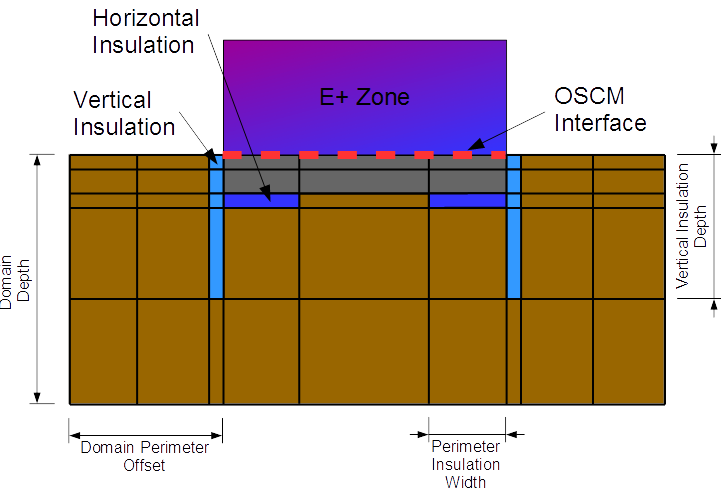
\includegraphics{media/image012.png}
\caption{In-grade configuration. \protect \label{fig:in-grade-configuration}}
\end{figure}

The in-grade slab option can be used to simulate situations when the upper slab surface is near the ground surface level. For this situation, slab's upper surface must interact with the zone via an OSCM boundary. Due to this, the FloorConstruction object for the zone floor must include a thin layer of the upper floor material. Horizontal and vertical insulation are modeled by the GroundDomain in this scenario. Horizontal insulation can be modeled as covering the full horizontal surface, or it can be limited to the perimeter regions only. In the latter case, the perimeter insulation width must be specified.

\begin{figure}[htbp]
\centering
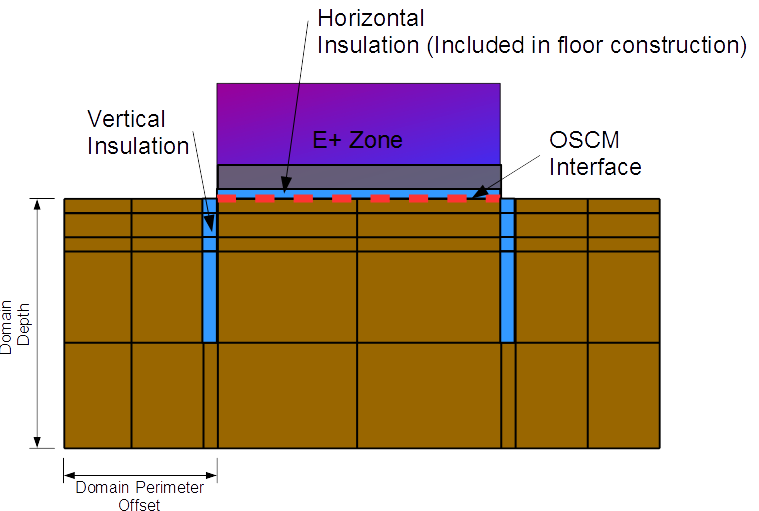
\includegraphics{media/image013.png}
\caption{On-grade configuration \protect \label{fig:on-grade-configuration}}
\end{figure}

The on-grade slab option can be used to simulate situations when the lower slab surface is near the ground surface level. In this situation, the entire floor must be included within the floor construction object. Vertical insulation is modeled by the GroundDomain in this scenario. Horizontal insulation can only be modeled as covering the full horizontal surface.

\subsubsection{Inputs}\label{inputs-16-006}

\paragraph{Field: Name}\label{field-name-8-009}

Alpha field used as a unique identifier for each ground domain.

\paragraph{Field: Ground Domain Depth}\label{field-ground-domain-depth}

Numeric field used to determine the depth of the simulation domain, in meters.

\paragraph{Field: Aspect Ratio}\label{field-aspect-ratio}

Numeric field used to define the height to width ratio of the slab.

\paragraph{Field: Perimeter Offset}\label{field-perimeter-offset}

Numeric field used to determine the distance from the slab perimeter to the domain perimeter, in meters.

\paragraph{Field: Soil Thermal Conductivity}\label{field-soil-thermal-conductivity-3}

The thermal conductivity of the soil, in W/m-K.

\paragraph{Field: Soil Density}\label{field-soil-density-3}

The bulk density of the soil, in kg/m3.

\paragraph{Field: Soil Specific Heat}\label{field-soil-specific-heat-3}

The specific heat of dry soil, in J/kg-K. If moisture is defined in this object, moisture and freezing effects are accounted for by varying the specific heat value.

\paragraph{Field: Soil Moisture Content Volume Fraction}\label{field-soil-moisture-content-volume-fraction-1}

A nominal value of soil moisture content to be used when evaluating soil thermal properties.

\paragraph{Field: Soil Moisture Content Volume Fraction at Saturation}\label{field-soil-moisture-content-volume-fraction-at-saturation-1}

A nominal value of soil moisture content when the soil is saturated, this is used in evaluating thermal properties of freezing soil.

\paragraph{Field: Type of Undisturbed Ground Temperature Object}\label{field-type-of-undisturbed-ground-temperature-object-000}

This is the type of undisturbed ground temperature object that is used to determine the ground temperature.

\paragraph{Field: Name of Undisturbed Ground Temperature Object}\label{field-name-of-undisturbed-ground-temperature-object-000}

This is the name of the undisturbed ground temperature object that is used to determine the ground temperature.

\paragraph{Field: Evapotranspiration Ground Cover Parameter}\label{field-evapotranspiration-ground-cover-parameter-1}

Numeric field specifies the ground cover effects used in the evapotranspiration model at the ground surface heat balance. The values range from 0 (solid, non-permeable ground surface) to 1.5 (wild growth).

\paragraph{Field: Slab Boundary Condition Model Name}\label{field-slab-boundary-condition-model-name}

This is the name of the other side boundary condition model used.

\paragraph{Field: Slab Location}\label{field-slab-location}

Alpha field indicates whether the slab is in-grade (top surface level with ground surface) or on-grade (bottoms surface level with ground surface). Options include ``ONGRADE'' and ``INGRADE''.

\paragraph{Field: Slab Material Name}\label{field-slab-material-name}

Name of the material object representing the slab material. Only applicable to in-grade situations.

\paragraph{Field: Horizontal Insulation}\label{field-horizontal-insulation}

Alpha field indicates whether horizontal insulation is present. Options include ``YES'' and ``NO''. Only applicable to in-grade situations.

\paragraph{Field: Horizontal Insulation Material Name}\label{field-horizontal-insulation-material-name}

Name of material object representing the horizontal slab insulation. Optional argument only required if horizontal insulation is present.

\paragraph{Field: Horizontal Insulation Extents}\label{field-horizontal-insulation-extents}

Alpha field indicates whether the horizontal slab insulation extends to cover the full horizontal area of the slab, or only covers the slab perimeter. Optional argument only required if horizontal insulation is present. Options include ``FULL'' and ``PERIMETER''.

\paragraph{Field: Perimeter Insulation Width}\label{field-perimeter-insulation-width}

Numeric field indicating the width of the perimeter insulation measured from the slab edge. Valid range from \textgreater{} 0 to \textless{} half of smallest slab width.

\paragraph{Field: Vertical Insulation}\label{field-vertical-insulation}

Alpha field indicates whether vertical insulation is present. Options include ``YES'' and ``NO''.

\paragraph{Field: Vertical Insulation Name}\label{field-vertical-insulation-name}

Name of material object representing the vertical slab insulation. Optional argument only required if vertical insulation is present.

\paragraph{Field: Vertical Insulation Depth}\label{field-vertical-insulation-depth}

Numeric field indicates the depth measured in meters from the ground surface to which the vertical perimeter insulation extends. Valid range from \textgreater{} Slab Thickness to \textless{} Domain Depth.

\paragraph{Field: Simulation Timestep}\label{field-simulation-timestep}

Alpha field indicating whether the domain will update temperatures at each zone timestep, or at hourly intervals. Options include ``timestep'' and ``hourly''.

An IDF example of an in-grade slab.

\begin{lstlisting}
Site:GroundDomain:Slab,
  IngradeCoupledSlab, !- Name
  5,                  !- Ground Domain Depth
  1,                  !- Aspect Ratio
  5,                  !- Domain Perimeter Offset
  1.8,                !- Soil Thermal Conductivity
  3200,               !- Soil Density
  836,                !- Soil Specific Heat
  30,                 !- Soil Moisture Content Volume Fraction
  50,                 !- Soil Moisture Content Volume Fraction at Saturation
  Site:GroundTemperature:Undisturbed:KusudaAchenbach, !- Type of Undisturbed Ground Temperature Object
  KATemps,            !- Name of Undisturbed Ground Temperature Object
  1,                  !- Evapotranspiration Ground Cover Parameter
  GroundCoupledOSCM,  !- Name of Floor Boundary Condition Model
  InGrade,            !- Slab Location (InGrade/OnGrade)
  Slab Material-In-grade, !- Slab Material Name
  Yes,                !- Horizontal Insulation
  Slab Insulation,    !- Horizontal Insulation Material Name
  Perimeter,          !- Full Horizontal or Perimeter Only
  1,                  !- Perimeter insulation width
  Yes,                !- Vertical Insulation
  Slab Insulation,    !- Vertical Insulation Name
  2,                  !- Vertical perimeter insulation depth from surface
  Hourly;             !- Simulation timestep
\end{lstlisting}

And IDF example of an on-grade slab

\begin{lstlisting}
Site:GroundDomain:Slab,
  OngradeCoupledSlab, !- Name
  5,                  !- Ground Domain Depth {m}
  1,                  !- Aspect Ratio
  5,                  !- Domain Perimeter Offset {m}
  1.8,                !- Soil Thermal Conductivity {W/m-K}
  3200,               !- Soil Density {kg/m3}
  836,                !- Soil Specific Heat {J/kg-K}
  30,                 !- Soil Moisture Content Volume Fraction
  50,                 !- Soil Moisture Content Volume Fraction at Saturation
  Site:GroundTemperature:Undisturbed:KusudaAchenbach, !- Type of Undisturbed Ground Temperature Object
  KATemps;            !- Name of Undisturbed Ground Temperature Object
  1,                  !- Evapotranspiration Ground Cover Parameter
  GroundCoupledOSCM,  !- Name of Floor Boundary Condition Model
  OnGrade,            !- Slab Location (InGrade/OnGrade)
  ,                   !- Slab Material Name
  ,                   !- Horizontal Insulation (Yes/No)
  ,                   !- Horizontal Insulation Material Name
  ,                   !- Full Horizontal or Perimeter Only
  ,                   !- Perimeter insulation width (m)
  Yes,                !- Vertical Insulation (Yes/No)
  Slab Insulation,    !- Vertical Insulation Name
  2,                  !- Vertical perimeter insulation depth from surface
  Hourly;             !- Simulation timestep. (Timestep/Hourly)</td>
\end{lstlisting}

\subsubsection{Outputs}\label{outputs-1-015}

The following output variables are available.

\begin{itemize}
\tightlist
\item
  Zone, Average, Zone Coupled Surface Heat Flux {[}W/m2{]}
\item
  Zone, Average, Zone Coupled Surface Temperature {[}C{]}
\end{itemize}

\paragraph{Zone Coupled Surface Heat Flux {[}W/m2{]}}\label{zone-coupled-surface-heat-flux-wm2}

This is the value of the heat flux provided to the GroundDomain as a boundary condition. This is calculated by taking the average heat flux of all surfaces coupled to the domain's SurfaceProperty:OtherSideConditionsModel model.

\paragraph{Zone Coupled Surface Temperature {[}C{]}}\label{zone-coupled-surface-temperature-c}

This is the value of the SurfaceProperty:OtherSideConditionsModel surface temperature. This is the temperature provided to the ground coupled surfaces as an outside boundary condition.

\subsection{Site:GroundDomain:Basement}\label{sitegrounddomainbasement}

This section documents the input object used to simulate ground coupled heat transfer with underground zones within EnergyPlus. Zone surfaces within EnergyPlus interact with the Site:GroundDomain:Basement object by utilizing the SurfaceProperty:OtherSideConditionsModel object. Two separate OSCM are required for the basement vertical and horizontal surfaces. Vertical wall surfaces will interact with the first OSCM while the horizontal floor surface will interact with the second OSCM. Basement floor and wall surfaces are constructed normally by using the BuildingSurface:Detailed object, with the outside boundary condition being the OtherSideConditionsModel for the basement floor or wall. The outside surface of the wall being the interface between the ground domain and the EnergyPlus zone. Horizontal and vertical ground insulation are simulated by the ground domain, and therefore should not be included in the wall and floor construction objects.

\begin{figure}[htbp]
\centering
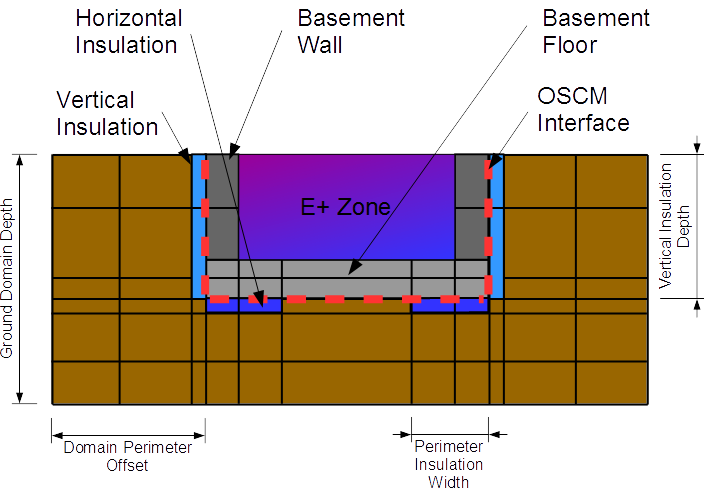
\includegraphics{media/image900.png}
\caption{Basement Configuration \protect \label{fig:basement-configuration}}
\end{figure}

\begin{lstlisting}
Site:GroundDomain:Basement,
  CoupledBasement,     !- Name
  10,                  !- Ground Domain Depth {m}
  1,                   !- Aspect ratio
  5,                   !- Perimeter offset {m}
  1.8,                 !- Soil Thermal Conductivity {W/m-K}
  3200,                !- Soil Density {kg/m3}
  836,                 !- Soil Specific Heat {J/kg-K}
  30,                  !- Soil Moisture Content Volume Fraction {percent}
  50,                  !- Soil Moisture Content Volume Fraction at Saturation {percent}
  Site:GroundTemperature:Undisturbed:KusudaAchenbach, !- Type of Undisturbed Ground Temperature Object
  KATemps,             !- Name of Undisturbed Ground Temperature Object
  1,                   !- Evapotranspiration Ground Cover Parameter
  BasementFloorOSCM,   !- Name of Basement Floor Boundary Condition Model
  Yes,                 !- Basement Horizontal Underfloor Insulation Present (Yes/No)
  Basement Insulation, !- Basement Horizontal Insulation Underfloor Material Name
  Full,                !- Full Horizontal or Perimeter Only (Full/Perimeter)
  ,                    !- Perimeter width (m)
  2.5,                 !- Depth of Basement Wall In Ground Domain {m}
  BasementWallOSCM,    !- Name of Basement Wall Boundary Condition Model
  Yes,                 !- Basement Wall Vertical Insulation Present(Yes/No)
  Basement Insulation, !- Basement Wall Vertical Insulation Material Name
  2.5,                 !- Vertical insulation depth from surface (m)
  Hourly;              !- Domain Update interval. (Timestep, Hourly)
  4;                   ! Mesh Density Parameter
\end{lstlisting}

\subsubsection{Inputs}\label{inputs-17-004}

\paragraph{Field: Name}\label{field-name-9-009}

Alpha field used as a unique identifier for each basement domain. Multiple basements domains can be simulated simultaneously, however, each domain must have a unique name. Additionally, despite the ability to simulate multiple domains simultaneously, these domains do not interact with each other and are treated as independent domains with boundary conditions given by the model parameters below.

\paragraph{Field: Ground Domain Depth}\label{field-ground-domain-depth-1}

Numeric field used to determine the depth of the simulation domain, in meters. A value of 10 meters is the default.

\paragraph{Field: Aspect Ratio}\label{field-aspect-ratio-1}

Numeric field, which is the ratio of basement length to width, used to determine the aspect ratio of the basement. This field along with the total basement floor area, which is taken as the combination of all surfaces connected to the floor OtherSideConditionsModel, are used to determine the size and shape of the basement domain. Aspect ratios and the inverse of aspect ratios should produce identical results. i.e. AR = 2 equals AR = 0.5. This field has units of meters/meters.

\paragraph{Field: Domain Perimeter Offset}\label{field-domain-perimeter-offset}

Numeric field used to determine the distance from the basement perimeter to the domain perimeter, in meters. A value of 5 is default.

\paragraph{Field: Soil Thermal Conductivity}\label{field-soil-thermal-conductivity-4}

The thermal conductivity of the soil, in W/m-K.

\paragraph{Field: Soil Density}\label{field-soil-density-4}

The bulk density of the soil, in kg/m3.

\paragraph{Field: Soil Specific Heat}\label{field-soil-specific-heat-4}

The specific heat of dry soil, in J/kg-K. If moisture is defined in this object, moisture and freezing effects are accounted for by varying the specific heat value.

\paragraph{Field: Soil Moisture Content Volume Fraction}\label{field-soil-moisture-content-volume-fraction-2}

A nominal value of soil moisture content to be used when evaluating soil thermal properties.

\paragraph{Field: Soil Moisture Content Volume Fraction at Saturation}\label{field-soil-moisture-content-volume-fraction-at-saturation-2}

A nominal value of soil moisture content when the soil is saturated, this is used in evaluating thermal properties of freezing soil.

\paragraph{Field: Type of Undisturbed Ground Temperature Object}\label{field-type-of-undisturbed-ground-temperature-object-1-000}

This is the type of undisturbed ground temperature object that is used to determine the ground temperature.

\paragraph{Field: Name of Undisturbed Ground Temperature Object}\label{field-name-of-undisturbed-ground-temperature-object-1-000}

This is the name of the undisturbed ground temperature object that is used to determine the ground temperature.

\paragraph{Field: Evapotranspiration Ground Cover Parameter}\label{field-evapotranspiration-ground-cover-parameter-2}

Numeric field specifies the ground cover effects used in the evapotranspiration model at the ground surface heat balance. The values range from 0 (solid, non-permeable ground surface) to 1.5 (wild growth). Model can be sensitive to variations in this parameter, especially in dry climates.

\paragraph{Field: Basement Floor Boundary Condition Model Name}\label{field-basement-floor-boundary-condition-model-name}

This is the name of the other side boundary condition model used for the basement floor surface.

\paragraph{Field: Horizontal Insulation}\label{field-horizontal-insulation-1}

Alpha field indicates whether horizontal insulation is present. Options include ``YES'' and ``NO''.

\paragraph{Field: Horizontal Insulation Name}\label{field-horizontal-insulation-name}

Name of material object representing the horizontal underfloor basement insulation. Optional argument only required if horizontal insulation is present.

\paragraph{Field: Horizontal Insulation Extents}\label{field-horizontal-insulation-extents-1}

Alpha field indicates whether the horizontal underfloor insulation extends to cover the full horizontal area of the basement floor, or only covers the basement floor perimeter. Optional argument only required if horizontal insulation is present. Options include ``FULL'' and ``PERIMETER''.

\paragraph{Field: Perimeter Insulation Width}\label{field-perimeter-insulation-width-1}

Numeric field indicating the width of the perimeter insulation measured from the basement floor edge. Valid range from \textgreater{} 0 to \textless{} half of smallest basement floor width.

\paragraph{Field: Basement Depth}\label{field-basement-depth}

Depth of basement floor surface referenced from the ground surface, in meters. This domain should be the distance from the ground surface down to the basement floor surface. In cases where the ground surface is below the main above-ground building level, a separate wall surface should be employed between the basement walls and the main level walls.

\paragraph{Field: Basement Wall Boundary Condition Model Name}\label{field-basement-wall-boundary-condition-model-name}

Name of the other side condition boundary model used for the basement walls.

\paragraph{Field: Vertical Insulation}\label{field-vertical-insulation-1}

Alpha field indicates whether vertical insulation is present. Options include ``YES'' and ``NO''.

\paragraph{Field: Vertical Insulation Name}\label{field-vertical-insulation-name-1}

Name of material object representing the vertical slab insulation. Optional argument only required if vertical insulation is present.

\paragraph{Field: Vertical Insulation Depth}\label{field-vertical-insulation-depth-1}

Numeric field indicates the depth measured in meters from the ground surface to which the vertical perimeter insulation extends. Valid range from \textgreater{} 0 to \textless{} Basement Depth.

\paragraph{Field: Simulation Timestep}\label{field-simulation-timestep-1}

Alpha field indicating whether the domain will update temperatures at each zone timestep, or at hourly intervals. Options include ``timestep'' and ``hourly''.

\paragraph{Mesh Density Parameter}\label{mesh-density-parameter}

Integer field indicating the density of the finite difference ground domain cells between the basement and the far field boundaries. Default value is 4. Total number of ground domain cells, insulation cells, and ground surface cells are indicated as outputs to the eio file.

\subsubsection{Outputs}\label{outputs-2-013}

The following output variables are available.

\begin{itemize}
\item
  Wall Interface Heat Flux
\item
  Wall Interface Temperature
\item
  Floor Interface Heat Flux
\item
  Floor Interface Temperature
\end{itemize}

\paragraph{Wall Interface Heat Flux {[}W/m2{]}}\label{wall-interface-heat-flux-wm2}

This is the value of the heat flux provided to ground domain as a boundary condition for the basement walls. Should be equal to the basement wall outside heat flux.

\paragraph{Wall Interface Temperature {[}C{]}}\label{wall-interface-temperature-c}

This is the value of the SurfaceProperty:OtherSideConditionsModel surface temperature. This is the temperature provided to the basement wall surfaces as an outside boundary condition.

\paragraph{Floor Interface Heat Flux {[}W/m2{]}}\label{floor-interface-heat-flux-wm2}

This is the value of the heat flux provided to ground domain as a boundary condition for the basement floor. Should be equal to the basement floor outside heat flux.

\paragraph{Floor Interface Temperature {[}C{]}}\label{floor-interface-temperature-c}

This is the value of the SurfaceProperty:OtherSideConditionsModel surface temperature. This is the temperature provided to the ground coupled floor surfaces as an outside boundary condition.

\subsection{Site:GroundTemperature:FCfactorMethod}\label{sitegroundtemperaturefcfactormethod}

Site:GroundTemperature:FCfactorMethod is used only by the underground walls or slabs-on-grade or underground floors defined with C-factor (Construction:CfactorUndergroundWall) and F-factor (Construction:FfactorGroundFloor) method for code compliance calculations where detailed construction layers are unknown. Only one such ground temperature object can be included. The monthly ground temperatures for this object are close to the monthly outside air temperatures delayed by three months. If user does not input this object in the IDF file, it will be defaulted to the 0.5m set of monthly ground temperatures from the weather file if they are available. Entering these will also overwrite any ground temperatures from the weather file in the F and C factor usage. If neither is available, an error will result.

\subsubsection{Inputs}\label{inputs-18-004}

\paragraph{Field: Month Temperature(s) -- 12 fields in all}\label{field-month-temperatures-12-fields-in-all-3}

Each numeric field is the monthly ground temperature (degrees Celsius) used for the indicated month (January = 1\(^{st}\) field, February = 2\(^{nd}\) field, etc.)

And, the IDF example:

\begin{lstlisting}
Site:GroundTemperature:FCfactorMethod,  9.5, 3.5, -0.7, -1.7, -0.6, 3.6, 9.3, 14, 18.2, 22.7, 21.2, 16.8;
\end{lstlisting}

\subsection{Site:GroundReflectance}\label{sitegroundreflectance}

Ground reflectance values are used to calculate the ground reflected solar amount. This fractional amount (entered monthly) is used in this equation:

\begin{equation}
\rm{GroundReflectedSolar} = \left( \rm{BeamSolar} \cdot cos \left( \rm{SunZenithAngle} \right) + \rm{DiffuseSolar} \right) \cdot \rm{GroundReflectance}
\end{equation}

Of course, the Ground Reflected Solar is never allowed to be negative. The ground reflectance can be further modified when snow is on the ground by the Snow Ground Reflectance Modifier. To use no ground reflected solar in your simulation, enter 0.0 for each month.

\subsubsection{Inputs}\label{inputs-19-003}

\paragraph{Field: Month Average Ground Reflectance(s) -- 12 fields in all}\label{field-month-average-ground-reflectances-12-fields-in-all}

Each numeric field is the monthly average reflectivity of the ground used for the indicated month (January = 1\(^{st}\) field, February = 2\(^{nd}\) field, etc.)

And use in an IDF:

\begin{lstlisting}
Site:GroundReflectance,
  0.600,     !January Ground Reflectance
  0.600,     !February Ground Reflectance
  0.400,     !March Ground Reflectance
  0.300,     !April Ground Reflectance
  0.200,     !May Ground Reflectance
  0.200,     !June Ground Reflectance
  0.200,     !July Ground Reflectance
  0.200,     !August Ground Reflectance
  0.200,     !September Ground Reflectance
  0.200,     !October Ground Reflectance
  0.300,     !November Ground Reflectance
  0.400;     !December Ground Reflectance
\end{lstlisting}

\subsection{Site:GroundReflectance:SnowModifier}\label{sitegroundreflectancesnowmodifier}

It is generally accepted that snow resident on the ground increases the basic ground reflectance. EnergyPlus allows the user control over the snow ground reflectance for both ``normal ground reflected solar'' calculations (see above) and snow ground reflected solar modified for daylighting. These are entered under this object and both default to 1 (same as normal ground reflectance -- no special case for snow which is a conservative approach).

\subsubsection{Inputs}\label{inputs-20-003}

\paragraph{Field: Ground Reflected Solar Modifier}\label{field-ground-reflected-solar-modifier}

This field is a decimal number which is used to modified the basic monthly ground reflectance when snow is on the ground (from design day input or weather data values).

\begin{equation}
\rm{GroundReflectance}_{\rm{used}} = \rm{GroundReflectance} \cdot \rm{Modifier}_{\rm{Snow}}
\end{equation}

The actual Ground Reflectance is limited to {[}0.0,1.0{]}.

\paragraph{Field: Daylighting Ground Reflected Solar Modifier}\label{field-daylighting-ground-reflected-solar-modifier}

This field is a decimal number which is used to modified the basic monthly ground reflectance when snow is on the ground (from design day input or weather data values).

\begin{equation}
\rm{DaylightingGroundReflectance}_{\rm{used}} = \rm{GroundReflectance} \cdot \rm{Modifier}_{\rm{Snow}}
\end{equation}

The actual Ground Reflectance is limited to {[}0.0,1.0{]}.

An IDF example:

\begin{lstlisting}
Site:GroundReflectance:SnowModifier,
  1.0;       !- Ground Reflected Solar Modifier
\end{lstlisting}

Outputs will show both the inputs from the above object as well as monthly values for both Snow Ground Reflectance and Snow Ground Reflectance for Daylighting.

\subsection{Site:WaterMainsTemperature}\label{sitewatermainstemperature}

The Site:WaterMainsTemperature object is used to calculate water temperatures delivered by underground water main pipes. The mains temperatures are used as default, make-up water temperature inputs for several plant objects, including: \textbf{WaterUse:Equipment, WaterUse:Connections, WaterHeater:Mixed} and \textbf{WaterHeater:Stratified}. The mains temperatures are also used in the water systems objects to model the temperature of cold water supplies.

Water mains temperatures are a function of outdoor climate conditions and vary with time of year. A correlation has been formulated to predict water mains temperatures based on two weather inputs:

\begin{itemize}
\item
  average annual outdoor air temperature (dry-bulb)
\item
  maximum difference in monthly average outdoor air temperatures
\end{itemize}

These values can be easily calculated from annual weather data using a spreadsheet or from the ``.stat'' file available with the EnergyPlus weather files at \href{http://www.energyplus.gov}{www.energyplus.gov}. Monthly statistics for dry-bulb temperatures are shown with daily averages. The daily averages are averaged to obtain the annual average. The maximum and minimum daily average are subtracted to obtain the maximum difference. For more information on the water mains temperatures correlation, see the \emph{EnergyPlus Engineering Document}.

Alternatively, the Site:WaterMainsTemperature object can read values from a schedule. This is useful for measured data or when water comes from a source other than buried pipes, e.g., a river or lake.

If there is no Site:WaterMainsTemperature object in the input file, a default constant value of 10 C is assumed.

\subsubsection{Inputs}\label{inputs-21-003}

\paragraph{Field: Calculation Method}\label{field-calculation-method}

This field selects the calculation method and must have the keyword Schedule or Correlation.

\paragraph{Field: Schedule Name}\label{field-schedule-name-003}

If the calculation method is Schedule, the water mains temperatures are read from the schedule referenced by this field. If the calculation method is Correlation, this field is ignored.

\paragraph{Field: Annual Average Outdoor Air Temperature}\label{field-annual-average-outdoor-air-temperature}

If the calculation method is Correlation, this field is used in the calculation as the annual average outdoor air temperature (dry-bulb) {[}C{]}. If the calculation method is Schedule, this field is ignored.

\paragraph{Field: Maximum Difference In Monthly Average Outdoor Air Temperatures}\label{field-maximum-difference-in-monthly-average-outdoor-air-temperatures}

If the calculation method is Correlation, this field is used in the calculation as the maximum difference in monthly average outdoor air temperatures {[}\(\Delta\)C{]}. If the calculation method is Schedule, this field is ignored.

\begin{lstlisting}
Site:WaterMainsTemperature,
  Correlation,  !- Calculation Method {SCHEDULE | CORRELATION}
  ,             !- Schedule Name
  9.69,         !- Annual Average Outdoor Air Temperature {C}
  28.1;         !- Maximum Difference In Monthly Average Outdoor Air Temperatures {deltaC}
\end{lstlisting}

\subsection{Site:Precipitation}\label{siteprecipitation}

The Site:Precipitation object is used to describe the amount of water precipitation at the building site over the course of the simulation run period. Precipitation includes both rain and the equivalent water content of snow. Precipitation is not yet described well enough in the many building weather data files. So this object can be used to provide the data using Schedule objects that define rates of precipitation in meters per hour.

A set of schedules for site precipitation have been developed for USA weather locations and are provided with EnergyPlus in the data set called PrecipitationSchedulesUSA.idf. The user can develop schedules however they want. The schedules in the data set were developed using EnergyPlus' weather file (EPW) observations and the average monthly precipitation for the closest weather site provided by NOAA. EPW files for the USA that were based on TMY or TMY2 include weather observations for Light/Moderate/Heavy rainfall, however most international locations do not include these observations. The values were modeled by taking the middle of the ranges quoted in the EPW data dictionary. The assumed piecewise function is shown below.

\begin{equation}
\rm{Amount} \, (m/hour) = \, \left\{
  \begin{array}{*{20}{c}}
    \rm{Light} = 0.0125 \\
    \rm{Moderate} = 0.052 \\
    \rm{Heavy} = 0.1
  \end{array}
\right.
\end{equation}

The values were inserted on hour by hour basis for the month based on the observations. Then each month was rescaled to meet the average precipitation for the month based on the 30-year average (1971-2000) provided by the NOAA/NCDC. Therefore, the flags in the EPW file match the precipitation schedules for the USA. Note that summing the average monthly precipitation values will not give you the average yearly precipitation. The resulting value may be lower or higher than the average yearly value.

Once the typical rainfall pattern and rates are scheduled, the Site:Precipitation object provides a method of shifting the total rainfall up or down for design purposes. Wetter or drier conditions can be modeled by changing the Design Annual Precipitation although the timing of precipitation throughout the year will not be changed.

\subsubsection{Inputs}\label{inputs-22-002}

\paragraph{Field: Precipitation Model Type}\label{field-precipitation-model-type}

Choose rainfall modeling options. Only available option is ScheduleAndDesignLevel.

\paragraph{Field: Design Level for Total Annual Precipitation}\label{field-design-level-for-total-annual-precipitation}

Magnitude of total precipitation for an annual period to be used in the model. Value selected by the user to correspond with the amount of precipitation expected or being assumed for design purposes. The units are in meters. This field works with the following two fields to allow easily shifting the amounts without having to generate new schedules.

\paragraph{Field: Precipitation Rate Schedule Name}\label{field-precipitation-rate-schedule-name}

Name of a schedule defined elsewhere that describes the rate of precipitation. The precipitation rate schedule is analogous to weather file data. However, weather files for building simulation do not currently contain adequate data for such calculations. Therefore, EnergyPlus schedules are used to enter the pattern of precipitation events. The values in this schedule are the average rate of precipitation in meters per hour. The integration of these values over an annual schedule should equal the nominal annual precipitation.

\paragraph{Field: Average Total Annual Precipitation}\label{field-average-total-annual-precipitation}

Magnitude of annual precipitation associated with the rate schedule. This value is used to normalize the precipitation.

IDF example:

\begin{lstlisting}
Site:Precipitation,
  ScheduledAndDesignLevel, !- Precipitation Model Type
  0.75,                    !- Design Level Total Annual Precipitation {m/yr}
  PrecipitationSchd,       !- Schedule Name for Precipitation Rates
  0.80771;                 !- Average Total Annual Precipitation {m/yr}
\end{lstlisting}

\subsection{RoofIrrigation}\label{roofirrigation}

The RoofIrrigation object is used to describe the amount of irrigation on the ecoroof surface over the course of the simulation runperiod. This object is used to provide irrigation data using Schedule objects that define rates of irrigation in meters per hour. These schedules can be one of two types: Schedule, or SmartSchedule.

\subsubsection{Inputs}\label{inputs-23-002}

\paragraph{Field: Irrigation Model Type}\label{field-irrigation-model-type}

Choose irrigation modeling options. Available options are \textbf{Schedule} and \textbf{SmartSchedule}. The \textbf{Schedule} type is used to force an irrigation schedule regardless of the current moisture state of the soil. The \textbf{SmartSchedule} type allows the precipitation schedule to be overridden if the current moisture state of the soil is greater than 40\% saturated.

\paragraph{Field: Irrigation Rate Schedule Name}\label{field-irrigation-rate-schedule-name}

Name of a schedule defined elsewhere that describes the rate of irrigation. The values in this schedule are the average rate of irrigation in meters per hour.

\paragraph{Field: Irrigation Maximum Saturation Threshold}\label{field-irrigation-maximum-saturation-threshold}

Used with the SmartSchedule option in the Irrigation Model Type field to override the default 40\% saturation limit for turning off the irrigation: values of 0 to 100 (percent) can be entered with 40\% being the default.

IDF example:

\begin{lstlisting}
RoofIrrigation,
  Schedule,       !- Irrigation Model Type
  IrrigationSchd; !- Schedule Name for Irrigation Rates
\end{lstlisting}

\subsection{Solar and Visible Spectrum Objects}\label{solar-and-visible-spectrum-objects}

The next two objects enable users to enter solar and visible spectrum which is used to calculate the thermal and visual performance of windows if their glazings are defined with full spectral data. EnergyPlus versions 8.0 and older hard-wired the solar and visible spectrum. The solar spectrum assumes air mass 1.5 terrestrial solar global spectral irradiance values (W/m2-micron) on a 37o tilted surface, based on ISO 9845-1 and ASTM E 892; derived from Optics5 data file ISO-9845GlobalNorm.std, 10-14-99. The visible/photopic spectrum is based on CIE 1931 observer; ISO/CIE 10527, CIE Standard Calorimetric Observers; derived from Optics5 data file ``CIE 1931 Color Match from E308.txt'', which is the same as WINDOW4 file Cie31t.dat.

\subsection{Site:SolarAndVisibleSpectrum}\label{sitesolarandvisiblespectrum}

The SolarAndVisibleSpectrum object is used to specify the solar and visible spectrum data which is used as spectral weighting function to calculate the window performance (transmittance and absorptance) in EnergyPlus. This is a unique object, if it is missing from an IDF file, the default (same as EnergyPlus version 8.0) solar and visible spectrum data will be used.

\subsubsection{Inputs}\label{inputs-24-001}

\paragraph{Field: Name}\label{field-name-10-008}

This field specifies the name of the SolarAndVisibleSpectrum object.

\paragraph{Field: Spectrum Data Method}\label{field-spectrum-data-method}

This field specifies the method used to enter the spectrum data. Two choices are available: Default and UserDefined. The choice Default will continue to use the hard-wired spectrum data in EnergyPlus (for backward compatibility). The choice UserDefined allows users to specify custom solar and visible spectrum data. The default choice is Default.

\paragraph{Field: Solar Spectrum Data Name}\label{field-solar-spectrum-data-name}

This field is required if the Spectrum Data Method is set to UserDefined. This field references a spectrum dataset for solar.

\paragraph{Field: Visible Spectrum Data Name}\label{field-visible-spectrum-data-name}

This field is required if the Spectrum Data Method is set to UserDefined. This field references a spectrum dataset for visible.

IDF example:

\begin{lstlisting}
Site:SolarAndVisibleSpectrum,
  LocalSpectrum,            !- Name
  UserDefined,              !- Spectrum Data Method: Default, UserDefined
  SolarSpectrum,            !- Solar Spectrum Data Object Name
  VisibleSpectrum;          !- Visible Spectrum Data Object
\end{lstlisting}

\subsection{Site:SpectrumData}\label{sitespectrumdata}

The Site:SpectrumData object holds the user defined solar or visible spectrum data. For solar spectrum, up to 107 pairs of (wavelength, spectrum) can be entered. For visible spectrum, up to 81 pairs can be entered.

\subsubsection{Inputs}\label{inputs-25-001}

\paragraph{Field: Name}\label{field-name-11-007}

This field specifies the name of the SpectrumData object. The name must be unique across all SpectrumData objects.

\paragraph{Field: Spectrum Data Type}\label{field-spectrum-data-type}

This field specifies the type of spectrum data. Choices are Solar and Visible.

\paragraph{Field: Wavelength \textless{}n\textgreater{}}\label{field-wavelength-n}

This field specifies the nth wavelength in micron.

\paragraph{Field: Spectrum \textless{}n\textgreater{}}\label{field-spectrum-n}

This field specifies the nth spectrum corresponding to the nth wavelength.

IDF example:

\begin{lstlisting}
Site:SpectrumData,
  SolarSpectrum, !- Name
  Solar,         !- Spectrum Data Type
  0.3,0,         !- up to 107 pair of (wavelength, spectrum)
  0.305,3.4,
  0.31,15.6,
  0.315,41.1,
  0.32,71.2,
  0.325,100.2,
  0.33,152.4,
  0.335,155.6,
  0.34,179.4,
  0.345,186.7,
  0.35,212,
  0.36,240.5,
  0.37,324,
  0.38,362.4,
  ...;
\end{lstlisting}

\subsubsection{Outputs}\label{outputs-3-011}

Climate related variables appear in two places for EnergyPlus outputs. Certain objects that are invariant throughout a simulation period have lines appear in the eplusout.eio file. For descriptions of this reporting, please see the Output Details and Examples document.

\subsubsection{Outputs}\label{outputs-4-008}

Variables related to ambient environment data are available at timestep and higher resolutions. Below is a variable dictionary of these variables and subsequent definitions:

\begin{itemize}
\item
  Zone,Average,Site Outdoor Air Drybulb Temperature {[}C{]}
\item
  Zone,Average,Site Outdoor Air Dewpoint Temperature {[}C{]}
\item
  Zone,Average,Site Outdoor Air Wetbulb Temperature {[}C{]}
\item
  Zone,Average,Site Outdoor Air Humidity Ratio {[}kgWater/kgAir{]}
\item
  Zone,Average,Site Outdoor Air Relative Humidity {[}\%{]}
\item
  Zone,Average,Site Outdoor Air Barometric Pressure {[}Pa{]}
\item
  Zone,Average,Site Wind Speed {[}m/s{]}
\item
  Zone,Average,Site Wind Direction {[}deg{]}
\item
  Zone,Average,Site Sky Temperature {[}C{]}
\item
  Zone,Average,Site Horizontal Infrared Radiation Rate per Area {[}W/m2{]}
\item
  Zone,Average,Site Diffuse Solar Radiation Rate per Area {[}W/m2{]}
\item
  Zone,Average,Site Direct Solar Radiation Rate per Area {[}W/m2{]}
\item
  Zone,Sum,Site Precipitation Depth {[}m{]}
\item
  Zone,Average,Site Ground Reflected Solar Radiation Rate per Area {[}W/m2{]}
\item
  Zone,Average,Site Ground Temperature {[}C{]}
\item
  Zone,Average,Site Surface Ground Temperature {[}C{]}
\item
  Zone,Average,Site Deep Ground Temperature {[}C{]}
\item
  Zone,Average,Site Simple Factor Model Ground Temperature {[}C{]}
\item
  Zone,Average,Site Outdoor Air Enthalpy {[}J/kg{]}
\item
  Zone,Average,Site Outdoor Air Density {[}kg/m3{]}
\item
  Zone,Average,Site Solar Azimuth Angle {[}deg{]}
\item
  Zone,Average,Site Solar Altitude Angle {[}deg{]}
\item
  Zone,Average,Site Solar Hour Angle {[}deg{]}
\item
  Zone,Average,Site Rain Status {[]}
\item
  Zone,Average,Site Snow on Ground Status {[]}
\item
  Zone,Average,Site Exterior Horizontal Sky Illuminance {[}lux{]}
\item
  Zone,Average,Site Exterior Horizontal Beam Illuminance {[}lux{]}
\item
  Zone,Average,Site Exterior Beam Normal Illuminance {[}lux{]}
\item
  Zone,Average,Site Sky Diffuse Solar Radiation Luminous Efficacy {[}lum/W{]}
\item
  Zone,Average,Site Beam Solar Radiation Luminous Efficacy {[}lum/W{]}
\item
  Zone,Average,Site Daylighting Model Sky Clearness {[]}
\item
  Zone,Average,Sky Brightness for Daylighting Calculation {[]}
\item
  Zone,Average,Site Daylight Saving Time Status {[]}
\item
  Zone,Average,Site Day Type Index {[]}
\item
  Zone,Average,Site Mains Water Temperature {[}C{]}
\item
  HVAC,Average,Site Precipitation Rate {[}m/s{]}
\item
  HVAC,Sum,Site Precipitation Depth {[}m{]}
\item
  HVAC,Sum,Water System Roof Irrigation Scheduled Depth{[}m{]}
\item
  HVAC,Sum,Water System Roof Irrigation Actual Depth{[}m{]}
\end{itemize}

Note that these data values may be interpolated from ``hour'' points (ref: Weather Data Hourly Interpolation). Most of the data values represent the ``average'' over the reporting resolution period.

\paragraph{Site Outdoor Air Drybulb Temperature {[}C{]}}\label{site-outdoor-air-drybulb-temperature-c}

This is the outdoor dry-bulb temperature in degrees C.

\paragraph{Site Outdoor Air Dewpoint Temperature {[}C{]}}\label{site-outdoor-air-dewpoint-temperature-c}

This is the outdoor dewpoint temperature in degrees C.

\paragraph{Site Outdoor Air Wetbulb Temperature {[}C{]}}\label{site-outdoor-air-wetbulb-temperature-c}

The outdoor wet-bulb temperature is derived (at the timestep) from the values for dry-bulb temperature, humidity ratio and barometric pressure.

\paragraph{Site Outdoor Air Humidity Ratio {[}kgWater/kgAir{]}}\label{site-outdoor-air-humidity-ratio-kgwaterkgair}

The outdoor humidity ratio is derived (at the timestep) from the dry-bulb temperature, relative humidity and barometric pressure.

\paragraph{Site Outdoor Air Relative Humidity {[}\%{]}}\label{site-outdoor-air-relative-humidity}

This is the outdoor relative humidity expressed in percent.

\paragraph{Site Outdoor Air Barometric Pressure {[}Pa{]}}\label{site-outdoor-air-barometric-pressure-pa}

This is the atmospheric/barometric pressure in Pa.

\paragraph{Site Wind Speed {[}m/s{]}}\label{site-wind-speed-ms}

This is the outdoor wind speed in m/s.

\paragraph{Site Wind Direction {[}deg{]}}\label{site-wind-direction-deg}

This is the wind direction (N = 0, E = 90, S = 180, W = 270).

\paragraph{Site Sky Temperature {[}C{]}}\label{site-sky-temperature-c}

The sky temperature is derived from horizontal infrared radiation intensity. It is expressed in degrees C. The default calculation is shown below but this value may be modified by the WeatherProperty:SkyTemperature object. Note that Sigma is the Stefan-Boltzmann constant in the following equation:

\begin{equation}
Sky\;Temperature = {\left( {\frac{{Horizontal\;IR}}{{Sigma}}} \right)^{\frac{1}{4}}} - {273.15_{Conversion\;from\;Kelvin\;to\;Centigrade}}
\end{equation}

\paragraph{Site Horizontal Infrared Radiation Rate per Area {[}W/m2{]}}\label{site-horizontal-infrared-radiation-rate-per-area-wm2}

The horizontal infrared radiation intensity is expressed in W/m\(^{2}\) based, if missing from the weather file, on opaque sky cover, sky emissivity, temperature and other factors. The general calculation of Site Horizontal Infrared Radiation Rate per Area is discussed in both the Engineering Reference and the Auxiliary Programs document.

\paragraph{Site Diffuse Solar Radiation Rate per Area {[}W/m2{]}}\label{site-diffuse-solar-radiation-rate-per-area-wm2}

Diffuse solar is the amount of solar radiation in W/m\(^{2}\) received from the sky (excluding the

solar disk) on a horizontal surface.

\paragraph{Site Direct Solar Radiation Rate per Area {[}W/m2{]}}\label{site-direct-solar-radiation-rate-per-area-wm2}

Site Direct Solar Radiation Rate per Area is amount of solar radiation in W/m\(^{2}\) received within a 5.7° field of view centered on the sun. This is also known as Beam Solar.

\paragraph{Site Precipitation Depth {[}m{]}}\label{site-precipitation-depth-m}

This is the amount of liquid precipitation (m). The source of this field may be the weather file or the Site:Precipitation object. The weather file values are in millimeters, but the report here is in meters. Two separate entities are displayed -- from the weather file the key value is ``Environment''; from the Site:Precipitation object the key value is Site:Precipitation.

If the weather file does not have a liquid precipitation field but does have the present weather fields, then a heuristic calculation is attempted for both flagging when it is raining and the amount of precipitation. If the weather file does have liquid precipitation fields, then the output (e.g. monthly) can be compared with the weather file stat file.

\paragraph{Site Ground Reflected Solar Radiation Rate per Area {[}W/m2{]}}\label{site-ground-reflected-solar-radiation-rate-per-area-wm2}

The ground reflected solar amount (W/m\(^{2}\)) is derived from the Beam Solar, Diffuse Solar, User specified Ground Reflectance (for month) and Solar Altitude Angle:

\begin{multline}
  \rm{Groundreflectedsolar}
  \\
  = \left( \rm{Beamsolar} \cdot cos \left( \rm{SolarAltitudeAngle} \right) + \rm{Diffusesolar} \right) \cdot \rm{Groundreflectance}_{\rm{month}}
\end{multline}

where if the calculation returns a value \textless{} 0.0, then 0.0 will be reported.

\paragraph{Site Ground Temperature {[}C{]}}\label{site-ground-temperature-c}

The ground temperature is reported in degrees C -- this is a user-specified input by month.

\paragraph{Site Surface Ground Temperature {[}C{]}}\label{site-surface-ground-temperature-c}

The ground temperature is reported in degrees C -- this is a user-specified input (object: Site:GroundTemperature:Shallow) by month.

\paragraph{Site Deep Ground Temperature {[}C{]}}\label{site-deep-ground-temperature-c}

The ground temperature is reported in degrees C -- this is a user-specified input (object: Site:GroundTemperature:Deep) by month.

\paragraph{Site Simple Factor Model Ground Temperature {[}C{]}}\label{site-simple-factor-model-ground-temperature-c}

The Site Simple Factor Model Ground Temperature is reported in degrees C -- this is a user-specified input (object: Site:GroundTemperature:FCfactorMethod) by month or gleaned from the weather file as noted in the description of the object.

\paragraph{Site Outdoor Air Enthalpy {[}J/kg{]}}\label{site-outdoor-air-enthalpy-jkg}

Outdoor enthalpy is derived at each timestep from the Site Outdoor Air Drybulb Temperature and the Site Outdoor Air Humidity Ratio. It is reported in J/kg.

\paragraph{Site Outdoor Air Density {[}kg/m3{]}}\label{site-outdoor-air-density-kgm3}

Outdoor air density is derived at each timestep from the Site Outdoor Air Barometric Pressure, the Outdoor Dry-bulb temperature and the Outdoor Humidity Ratio. It is reported in units kg/m\(^{3}\).

\paragraph{Site Solar Azimuth Angle {[}deg{]}}\label{site-solar-azimuth-angle-deg}

The Solar Azimuth Angle (f) is measured from the North (clockwise) and is expressed in degrees. This is shown more clearly in the following figure.

\begin{figure}[hbtp] % fig 9
\centering
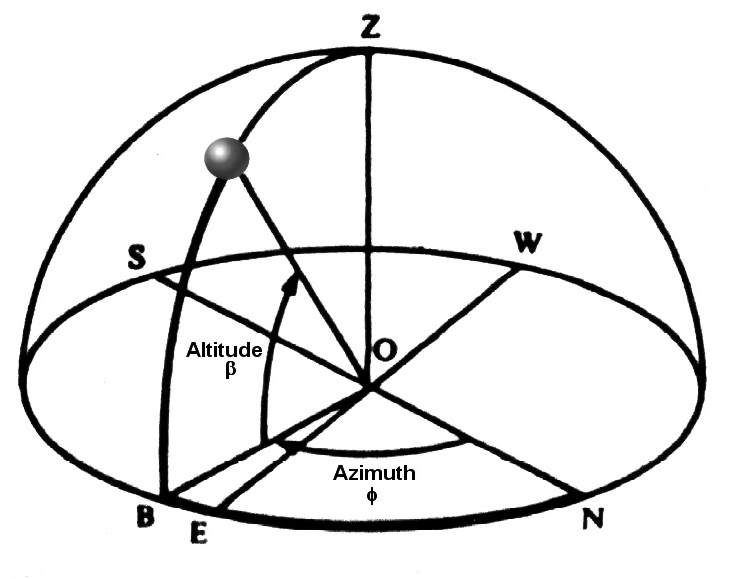
\includegraphics[width=0.9\textwidth, height=0.9\textheight, keepaspectratio=true]{media/image020.png}
\caption{Solar Position Illustration \protect \label{fig:solar-position-illustration}}
\end{figure}

\paragraph{Site Solar Altitude Angle {[}deg{]}}\label{site-solar-altitude-angle-deg}

The Solar Altitude Angle (b) is the angle of the sun above the horizontal (degrees).

\paragraph{Site Solar Hour Angle {[}deg{]}}\label{site-solar-hour-angle-deg}

The Solar Hour Angle (\emph{H}) gives the apparent solar time for the current time period (degrees). It is common astronomical practice to express the hour angle in hours, minutes and seconds of time rather than in degrees. You can convert the hour angle displayed from EnergyPlus to time by dividing by 15. (Note that 1 hour is equivalent to 15 degrees; 360° of the Earth's rotation takes place every 24 hours.) The relationship of angles in degrees to time is shown in the following table:

% table 6
\begin{longtable}[c]{@{}ll@{}}
\caption{Relationship of Angles (degrees) to Time \label{table:relationship-of-angles-degrees-to-time}} \tabularnewline
\toprule 
Unit of Angle & Equivalent time \tabularnewline
\midrule
\endfirsthead

\caption[]{Relationship of Angles (degrees) to Time} \tabularnewline
\toprule 
Unit of Angle & Equivalent time \tabularnewline
\midrule
\endhead

1 radian & 3.819719 hours \tabularnewline
1 degree & 4 minutes \tabularnewline
1 arcmin & 4 seconds \tabularnewline
1 arcsec & 0.066667 seconds \tabularnewline
\bottomrule
\end{longtable}

\paragraph{Site Rain Status {[]}}\label{site-rain-status}

This field shows whether or not (1 = yes, 0 = no) the weather shows ``raining''. For a Design Day, one can denote rain for the entire day but not timestep by timestep. Weather files may indicate rain for a single time interval. This is an ``averaged'' field -- thus a 1 shown for a time period (e.g. daily reporting) means that it was raining during each timestep of that period.

\paragraph{Site Snow on Ground Status {[]}}\label{site-snow-on-ground-status}

This field shows whether or not (1 = yes, 0 = no) the weather shows ``snow on the ground''. For a Design Day, one can denote snow for the entire day but not timestep by timestep. Weather files may indicate snow (snow depth) for a single time interval. This is an ``averaged'' field -- thus a 1 shown for a time period (e.g. daily reporting) means that there was snow on the ground during each timestep of that period.

\paragraph{Site Daylight Saving Time Status {[]}}\label{site-daylight-saving-time-status}

This field shows when daylight saving time (1 = yes, 0 = no) is in effect. Though shown as an average variable, this value is only set on a daily basis.

\paragraph{Site Day Type Index {[]}}\label{site-day-type-index}

This field shows what ``day type'' the current day is. Day types are (1 = Sunday, 2 = Monday, etc.) with Holiday = 8, SummerDesignDay = 9, WinterDesignDay = 10, CustomDay1 = 11, CustomDay2 = 12. Though shown as an average variable, this value is only set on a daily basis.

\paragraph{Site Mains Water Temperature {[}C{]}}\label{site-mains-water-temperature-c}

The value of the Water Mains Temperature is reported in C following the calculation shown in the Water Mains Temperature object.

\paragraph{Site Precipitation Rate {[}m/s{]}}\label{site-precipitation-rate-ms}

\paragraph{Site Precipitation Depth {[}m{]}}\label{site-precipitation-depth-m-1}

The rate and quantity of precipitation at the site. These outputs are only available if a Site Precipitation object is used. Precipitation is measured in meters.

\paragraph{Water System Roof Irrigation Scheduled Depth{[}m{]}}\label{water-system-roof-irrigation-scheduled-depthm}

This is the scheduled amount of irrigation for the green roof (ecoroof) based on the user input. Amount is measured in meters.

\paragraph{Water System Roof Irrigation Actual Depth{[}m{]}}\label{water-system-roof-irrigation-actual-depthm}

This is the actual amount of irrigation for the green roof (ecoroof) based on the scheduled user input and moisture state/saturation of the soil. Amount is measured in meters.

\subsection{Outputs for local temperature/wind speed calculations}\label{outputs-for-local-temperaturewind-speed-calculations}

Local atmospheric properties for outdoor air temperature and wind speed are separately calculated and reported for all zones, surfaces, and outdoor air nodes. The output variables are associated with their respective objects:

\begin{itemize}
\item
  Zone,Average,Zone Outdoor Air Drybulb Temperature {[}C{]}
\item
  Zone,Average,Zone Outdoor Air Wetbulb Temperature {[}C{]}
\item
  Zone,Average,Zone Outdoor Air Wind Speed {[}m/s{]}
\item
  Zone,Average,Surface Ext Outdoor Dry Bulb {[}C{]}
\item
  Zone,Average,Surface Ext Outdoor Wet Bulb {[}C{]}
\item
  Zone,Average,Surface Ext Wind Speed {[}m/s{]}
\item
  HVAC,Average,System Node Temperature {[}C{]}~~~~~~~ (for OUTDOOR AIR NODE object)
\end{itemize}

\subsubsection{Zone Outdoor Air Drybulb Temperature {[}C{]}}\label{zone-outdoor-air-drybulb-temperature-c}

The outdoor air dry-bulb temperature calculated at the height above ground of the zone centroid.

\subsubsection{Zone Outdoor Air Wetbulb Temperature {[}C{]}}\label{zone-outdoor-air-wetbulb-temperature-c}

The outdoor air wet-bulb temperature calculated at the height above ground of the zone centroid.

\subsubsection{Zone Outdoor Air Wind Speed {[}m/s{]}}\label{zone-outdoor-air-wind-speed-ms}

The outdoor wind speed calculated at the height above ground of the zone centroid.

\subsubsection{Surface Ext Outdoor Dry Bulb {[}C{]}}\label{surface-ext-outdoor-dry-bulb-c}

The outdoor air dry-bulb temperature calculated at the height above ground of the surface centroid.

\subsubsection{Surface Ext Outdoor Wet Bulb {[}C{]}}\label{surface-ext-outdoor-wet-bulb-c}

The outdoor air wet-bulb temperature calculated at the height above ground of the surface centroid.

\subsubsection{Surface Ext Wind Speed {[}m/s{]}}\label{surface-ext-wind-speed-ms}

The outdoor wind speed calculated at the height above ground of the surface centroid.

\subsubsection{System Node Temperature {[}C{]}}\label{system-node-temperature-c}

When reporting for the \textbf{OutdoorAir:Node} object, this is the outdoor air dry-bulb temperature calculated at the height above ground of the node, if height is specified in the input.
